\documentclass[twoside]{book}

% Packages required by doxygen
\usepackage{fixltx2e}
\usepackage{calc}
\usepackage{doxygen}
\usepackage[export]{adjustbox} % also loads graphicx
\usepackage{graphicx}
\usepackage[utf8]{inputenc}
\usepackage{makeidx}
\usepackage{multicol}
\usepackage{multirow}
\PassOptionsToPackage{warn}{textcomp}
\usepackage{textcomp}
\usepackage[nointegrals]{wasysym}
\usepackage[table]{xcolor}

% Font selection
\usepackage[T1]{fontenc}
\usepackage[scaled=.90]{helvet}
\usepackage{courier}
\usepackage{amssymb}
\usepackage{sectsty}
\renewcommand{\familydefault}{\sfdefault}
\allsectionsfont{%
  \fontseries{bc}\selectfont%
  \color{darkgray}%
}
\renewcommand{\DoxyLabelFont}{%
  \fontseries{bc}\selectfont%
  \color{darkgray}%
}
\newcommand{\+}{\discretionary{\mbox{\scriptsize$\hookleftarrow$}}{}{}}

% Page & text layout
\usepackage{geometry}
\geometry{%
  a4paper,%
  top=2.5cm,%
  bottom=2.5cm,%
  left=2.5cm,%
  right=2.5cm%
}
\tolerance=750
\hfuzz=15pt
\hbadness=750
\setlength{\emergencystretch}{15pt}
\setlength{\parindent}{0cm}
\setlength{\parskip}{0.2cm}
\makeatletter
\renewcommand{\paragraph}{%
  \@startsection{paragraph}{4}{0ex}{-1.0ex}{1.0ex}{%
    \normalfont\normalsize\bfseries\SS@parafont%
  }%
}
\renewcommand{\subparagraph}{%
  \@startsection{subparagraph}{5}{0ex}{-1.0ex}{1.0ex}{%
    \normalfont\normalsize\bfseries\SS@subparafont%
  }%
}
\makeatother

% Headers & footers
\usepackage{fancyhdr}
\pagestyle{fancyplain}
\fancyhead[LE]{\fancyplain{}{\bfseries\thepage}}
\fancyhead[CE]{\fancyplain{}{}}
\fancyhead[RE]{\fancyplain{}{\bfseries\leftmark}}
\fancyhead[LO]{\fancyplain{}{\bfseries\rightmark}}
\fancyhead[CO]{\fancyplain{}{}}
\fancyhead[RO]{\fancyplain{}{\bfseries\thepage}}
\fancyfoot[LE]{\fancyplain{}{}}
\fancyfoot[CE]{\fancyplain{}{}}
\fancyfoot[RE]{\fancyplain{}{\bfseries\scriptsize Generated on Sat Oct 24 2015 12\+:49\+:25 for Gravity\+Tanks by Doxygen }}
\fancyfoot[LO]{\fancyplain{}{\bfseries\scriptsize Generated on Sat Oct 24 2015 12\+:49\+:25 for Gravity\+Tanks by Doxygen }}
\fancyfoot[CO]{\fancyplain{}{}}
\fancyfoot[RO]{\fancyplain{}{}}
\renewcommand{\footrulewidth}{0.4pt}
\renewcommand{\chaptermark}[1]{%
  \markboth{#1}{}%
}
\renewcommand{\sectionmark}[1]{%
  \markright{\thesection\ #1}%
}

% Indices & bibliography
\usepackage{natbib}
\usepackage[titles]{tocloft}
\setcounter{tocdepth}{3}
\setcounter{secnumdepth}{5}
\makeindex

% Hyperlinks (required, but should be loaded last)
\usepackage{ifpdf}
\ifpdf
  \usepackage[pdftex,pagebackref=true]{hyperref}
\else
  \usepackage[ps2pdf,pagebackref=true]{hyperref}
\fi
\hypersetup{%
  colorlinks=true,%
  linkcolor=blue,%
  citecolor=blue,%
  unicode%
}

% Custom commands
\newcommand{\clearemptydoublepage}{%
  \newpage{\pagestyle{empty}\cleardoublepage}%
}


%===== C O N T E N T S =====

\begin{document}

% Titlepage & ToC
\hypersetup{pageanchor=false,
             bookmarks=true,
             bookmarksnumbered=true,
             pdfencoding=unicode
            }
\pagenumbering{roman}
\begin{titlepage}
\vspace*{7cm}
\begin{center}%
{\Large Gravity\+Tanks }\\
\vspace*{1cm}
{\large Generated by Doxygen 1.8.10}\\
\vspace*{0.5cm}
{\small Sat Oct 24 2015 12:49:25}\\
\end{center}
\end{titlepage}
\clearemptydoublepage
\tableofcontents
\clearemptydoublepage
\pagenumbering{arabic}
\hypersetup{pageanchor=true}

%--- Begin generated contents ---
\chapter{Namespace Index}
\section{Packages}
Here are the packages with brief descriptions (if available)\+:\begin{DoxyCompactList}
\item\contentsline{section}{\hyperlink{namespace_g_t_core}{G\+T\+Core} }{\pageref{namespace_g_t_core}}{}
\item\contentsline{section}{\hyperlink{namespace_g_t_core_1_1_camera}{G\+T\+Core.\+Camera} }{\pageref{namespace_g_t_core_1_1_camera}}{}
\item\contentsline{section}{\hyperlink{namespace_g_t_core_1_1_enemies}{G\+T\+Core.\+Enemies} }{\pageref{namespace_g_t_core_1_1_enemies}}{}
\item\contentsline{section}{\hyperlink{namespace_g_t_core_1_1_enviroment}{G\+T\+Core.\+Enviroment} }{\pageref{namespace_g_t_core_1_1_enviroment}}{}
\item\contentsline{section}{\hyperlink{namespace_g_t_core_1_1_general}{G\+T\+Core.\+General} }{\pageref{namespace_g_t_core_1_1_general}}{}
\item\contentsline{section}{\hyperlink{namespace_g_t_core_1_1_player}{G\+T\+Core.\+Player} }{\pageref{namespace_g_t_core_1_1_player}}{}
\item\contentsline{section}{\hyperlink{namespace_g_t_utils}{G\+T\+Utils} }{\pageref{namespace_g_t_utils}}{}
\end{DoxyCompactList}

\chapter{Hierarchical Index}
\section{Class Hierarchy}
This inheritance list is sorted roughly, but not completely, alphabetically\+:\begin{DoxyCompactList}
\item Mono\+Behaviour\begin{DoxyCompactList}
\item \contentsline{section}{G\+T\+Core.\+Camera.\+Camera\+Movement}{\pageref{class_g_t_core_1_1_camera_1_1_camera_movement}}{}
\item \contentsline{section}{G\+T\+Core.\+Enemies.\+Follow\+Bomb\+Movement}{\pageref{class_g_t_core_1_1_enemies_1_1_follow_bomb_movement}}{}
\item \contentsline{section}{G\+T\+Core.\+Enviroment.\+Bullet\+Parameters}{\pageref{class_g_t_core_1_1_enviroment_1_1_bullet_parameters}}{}
\item \contentsline{section}{G\+T\+Core.\+Enviroment.\+Planet\+Info}{\pageref{class_g_t_core_1_1_enviroment_1_1_planet_info}}{}
\item \contentsline{section}{G\+T\+Core.\+Enviroment.\+Satellite\+Movement}{\pageref{class_g_t_core_1_1_enviroment_1_1_satellite_movement}}{}
\item \contentsline{section}{G\+T\+Core.\+Enviroment.\+Spherical\+Gravity}{\pageref{class_g_t_core_1_1_enviroment_1_1_spherical_gravity}}{}
\item \contentsline{section}{G\+T\+Core.\+General.\+Actor\+Status}{\pageref{class_g_t_core_1_1_general_1_1_actor_status}}{}
\item \contentsline{section}{G\+T\+Core.\+General.\+Stick\+To\+Player}{\pageref{class_g_t_core_1_1_general_1_1_stick_to_player}}{}
\item \contentsline{section}{G\+T\+Core.\+Player.\+Canon\+Movement}{\pageref{class_g_t_core_1_1_player_1_1_canon_movement}}{}
\item \contentsline{section}{G\+T\+Core.\+Player.\+Player\+Movement}{\pageref{class_g_t_core_1_1_player_1_1_player_movement}}{}
\item \contentsline{section}{G\+T\+Core.\+Player.\+Player\+Shooting}{\pageref{class_g_t_core_1_1_player_1_1_player_shooting}}{}
\item \contentsline{section}{G\+T\+Core.\+Player.\+Stick\+To\+Planet}{\pageref{class_g_t_core_1_1_player_1_1_stick_to_planet}}{}
\end{DoxyCompactList}
\item Property\+Attribute\begin{DoxyCompactList}
\item \contentsline{section}{G\+T\+Utils.\+Bit\+Mask\+Attribute}{\pageref{class_g_t_utils_1_1_bit_mask_attribute}}{}
\end{DoxyCompactList}
\item Property\+Drawer\begin{DoxyCompactList}
\item \contentsline{section}{Enum\+Flags\+Attribute\+Drawer}{\pageref{class_enum_flags_attribute_drawer}}{}
\end{DoxyCompactList}
\item \contentsline{section}{G\+T\+Core.\+General.\+Actor\+Status.\+Transform\+Storage}{\pageref{class_g_t_core_1_1_general_1_1_actor_status_1_1_transform_storage}}{}
\end{DoxyCompactList}

\chapter{Class Index}
\section{Class List}
Here are the classes, structs, unions and interfaces with brief descriptions\+:\begin{DoxyCompactList}
\item\contentsline{section}{\hyperlink{class_g_t_core_1_1_general_1_1_actor_status}{G\+T\+Core.\+General.\+Actor\+Status} }{\pageref{class_g_t_core_1_1_general_1_1_actor_status}}{}
\item\contentsline{section}{\hyperlink{class_g_t_utils_1_1_bit_mask_attribute}{G\+T\+Utils.\+Bit\+Mask\+Attribute} }{\pageref{class_g_t_utils_1_1_bit_mask_attribute}}{}
\item\contentsline{section}{\hyperlink{class_g_t_core_1_1_enviroment_1_1_bullet_parameters}{G\+T\+Core.\+Enviroment.\+Bullet\+Parameters} }{\pageref{class_g_t_core_1_1_enviroment_1_1_bullet_parameters}}{}
\item\contentsline{section}{\hyperlink{class_g_t_core_1_1_camera_1_1_camera_movement}{G\+T\+Core.\+Camera.\+Camera\+Movement} \\*Controls the main camera movement behaviour }{\pageref{class_g_t_core_1_1_camera_1_1_camera_movement}}{}
\item\contentsline{section}{\hyperlink{class_g_t_core_1_1_player_1_1_canon_movement}{G\+T\+Core.\+Player.\+Canon\+Movement} }{\pageref{class_g_t_core_1_1_player_1_1_canon_movement}}{}
\item\contentsline{section}{\hyperlink{class_enum_flags_attribute_drawer}{Enum\+Flags\+Attribute\+Drawer} }{\pageref{class_enum_flags_attribute_drawer}}{}
\item\contentsline{section}{\hyperlink{class_g_t_core_1_1_enemies_1_1_follow_bomb_movement}{G\+T\+Core.\+Enemies.\+Follow\+Bomb\+Movement} \\*Defined the behaviour of the Follow\+Bomb enemy, this enemy is supposed to follow the player and explode once he is close enough or collides with the player }{\pageref{class_g_t_core_1_1_enemies_1_1_follow_bomb_movement}}{}
\item\contentsline{section}{\hyperlink{class_g_t_core_1_1_enviroment_1_1_planet_info}{G\+T\+Core.\+Enviroment.\+Planet\+Info} }{\pageref{class_g_t_core_1_1_enviroment_1_1_planet_info}}{}
\item\contentsline{section}{\hyperlink{class_g_t_core_1_1_player_1_1_player_movement}{G\+T\+Core.\+Player.\+Player\+Movement} }{\pageref{class_g_t_core_1_1_player_1_1_player_movement}}{}
\item\contentsline{section}{\hyperlink{class_g_t_core_1_1_player_1_1_player_shooting}{G\+T\+Core.\+Player.\+Player\+Shooting} }{\pageref{class_g_t_core_1_1_player_1_1_player_shooting}}{}
\item\contentsline{section}{\hyperlink{class_g_t_core_1_1_enviroment_1_1_satellite_movement}{G\+T\+Core.\+Enviroment.\+Satellite\+Movement} }{\pageref{class_g_t_core_1_1_enviroment_1_1_satellite_movement}}{}
\item\contentsline{section}{\hyperlink{class_g_t_core_1_1_enviroment_1_1_spherical_gravity}{G\+T\+Core.\+Enviroment.\+Spherical\+Gravity} }{\pageref{class_g_t_core_1_1_enviroment_1_1_spherical_gravity}}{}
\item\contentsline{section}{\hyperlink{class_g_t_core_1_1_player_1_1_stick_to_planet}{G\+T\+Core.\+Player.\+Stick\+To\+Planet} }{\pageref{class_g_t_core_1_1_player_1_1_stick_to_planet}}{}
\item\contentsline{section}{\hyperlink{class_g_t_core_1_1_general_1_1_stick_to_player}{G\+T\+Core.\+General.\+Stick\+To\+Player} }{\pageref{class_g_t_core_1_1_general_1_1_stick_to_player}}{}
\item\contentsline{section}{\hyperlink{class_g_t_core_1_1_general_1_1_actor_status_1_1_transform_storage}{G\+T\+Core.\+General.\+Actor\+Status.\+Transform\+Storage} }{\pageref{class_g_t_core_1_1_general_1_1_actor_status_1_1_transform_storage}}{}
\end{DoxyCompactList}

\chapter{File Index}
\section{File List}
Here is a list of all files with brief descriptions\+:\begin{DoxyCompactList}
\item\contentsline{section}{Assets/\+Debug\+Drawing\+Extension/\hyperlink{_debug_extension_8cs}{Debug\+Extension.\+cs} }{\pageref{_debug_extension_8cs}}{}
\item\contentsline{section}{Assets/\+Editor/\hyperlink{_bit_mask_drawer_8cs}{Bit\+Mask\+Drawer.\+cs} }{\pageref{_bit_mask_drawer_8cs}}{}
\item\contentsline{section}{Assets/\+Scripts/\+G\+T\+Core/\+Camera/\hyperlink{_camera_movement_8cs}{Camera\+Movement.\+cs} }{\pageref{_camera_movement_8cs}}{}
\item\contentsline{section}{Assets/\+Scripts/\+G\+T\+Core/\+Enemies/\hyperlink{_follow_bomb_movement_8cs}{Follow\+Bomb\+Movement.\+cs} }{\pageref{_follow_bomb_movement_8cs}}{}
\item\contentsline{section}{Assets/\+Scripts/\+G\+T\+Core/\+Enviroment/\hyperlink{_bullet_parameters_8cs}{Bullet\+Parameters.\+cs} }{\pageref{_bullet_parameters_8cs}}{}
\item\contentsline{section}{Assets/\+Scripts/\+G\+T\+Core/\+Enviroment/\hyperlink{_planet_info_8cs}{Planet\+Info.\+cs} }{\pageref{_planet_info_8cs}}{}
\item\contentsline{section}{Assets/\+Scripts/\+G\+T\+Core/\+Enviroment/\hyperlink{_satellite_movement_8cs}{Satellite\+Movement.\+cs} }{\pageref{_satellite_movement_8cs}}{}
\item\contentsline{section}{Assets/\+Scripts/\+G\+T\+Core/\+Enviroment/\hyperlink{_spherical_gravity_8cs}{Spherical\+Gravity.\+cs} }{\pageref{_spherical_gravity_8cs}}{}
\item\contentsline{section}{Assets/\+Scripts/\+G\+T\+Core/\+General/\hyperlink{_actor_status_8cs}{Actor\+Status.\+cs} }{\pageref{_actor_status_8cs}}{}
\item\contentsline{section}{Assets/\+Scripts/\+G\+T\+Core/\+General/\hyperlink{_stick_to_player_8cs}{Stick\+To\+Player.\+cs} }{\pageref{_stick_to_player_8cs}}{}
\item\contentsline{section}{Assets/\+Scripts/\+G\+T\+Core/\+Player/\hyperlink{_canon_movement_8cs}{Canon\+Movement.\+cs} }{\pageref{_canon_movement_8cs}}{}
\item\contentsline{section}{Assets/\+Scripts/\+G\+T\+Core/\+Player/\hyperlink{_player_movement_8cs}{Player\+Movement.\+cs} }{\pageref{_player_movement_8cs}}{}
\item\contentsline{section}{Assets/\+Scripts/\+G\+T\+Core/\+Player/\hyperlink{_player_shooting_8cs}{Player\+Shooting.\+cs} }{\pageref{_player_shooting_8cs}}{}
\item\contentsline{section}{Assets/\+Scripts/\+G\+T\+Core/\+Player/\hyperlink{_stick_to_planet_8cs}{Stick\+To\+Planet.\+cs} }{\pageref{_stick_to_planet_8cs}}{}
\item\contentsline{section}{Assets/\+Scripts/\+G\+T\+Utils/\hyperlink{_bit_mask_attribute_8cs}{Bit\+Mask\+Attribute.\+cs} }{\pageref{_bit_mask_attribute_8cs}}{}
\item\contentsline{section}{Assets/\+Scripts/\+G\+T\+Utils/\hyperlink{_draw_arrow_8cs}{Draw\+Arrow.\+cs} }{\pageref{_draw_arrow_8cs}}{}
\end{DoxyCompactList}

\chapter{Namespace Documentation}
\hypertarget{namespace_g_t_core}{}\section{G\+T\+Core Namespace Reference}
\label{namespace_g_t_core}\index{G\+T\+Core@{G\+T\+Core}}
\subsection*{Namespaces}
\begin{DoxyCompactItemize}
\item 
namespace \hyperlink{namespace_g_t_core_1_1_camera}{Camera}
\item 
namespace \hyperlink{namespace_g_t_core_1_1_enemies}{Enemies}
\item 
namespace \hyperlink{namespace_g_t_core_1_1_enviroment}{Enviroment}
\item 
namespace \hyperlink{namespace_g_t_core_1_1_general}{General}
\item 
namespace \hyperlink{namespace_g_t_core_1_1_player}{Player}
\end{DoxyCompactItemize}

\hypertarget{namespace_g_t_core_1_1_camera}{}\section{G\+T\+Core.\+Camera Namespace Reference}
\label{namespace_g_t_core_1_1_camera}\index{G\+T\+Core.\+Camera@{G\+T\+Core.\+Camera}}
\subsection*{Classes}
\begin{DoxyCompactItemize}
\item 
class \hyperlink{class_g_t_core_1_1_camera_1_1_camera_movement}{Camera\+Movement}
\begin{DoxyCompactList}\small\item\em Controls the main camera movement behaviour \end{DoxyCompactList}\end{DoxyCompactItemize}

\hypertarget{namespace_g_t_core_1_1_enemies}{}\section{G\+T\+Core.\+Enemies Namespace Reference}
\label{namespace_g_t_core_1_1_enemies}\index{G\+T\+Core.\+Enemies@{G\+T\+Core.\+Enemies}}
\subsection*{Classes}
\begin{DoxyCompactItemize}
\item 
class \hyperlink{class_g_t_core_1_1_enemies_1_1_follow_bomb_movement}{Follow\+Bomb\+Movement}
\begin{DoxyCompactList}\small\item\em Defined the behaviour of the Follow\+Bomb enemy, this enemy is supposed to follow the player and explode once he is close enough or collides with the player \end{DoxyCompactList}\end{DoxyCompactItemize}

\hypertarget{namespace_g_t_core_1_1_enviroment}{}\section{G\+T\+Core.\+Enviroment Namespace Reference}
\label{namespace_g_t_core_1_1_enviroment}\index{G\+T\+Core.\+Enviroment@{G\+T\+Core.\+Enviroment}}
\subsection*{Classes}
\begin{DoxyCompactItemize}
\item 
class \hyperlink{class_g_t_core_1_1_enviroment_1_1_bullet_parameters}{Bullet\+Parameters}
\item 
class \hyperlink{class_g_t_core_1_1_enviroment_1_1_planet_info}{Planet\+Info}
\item 
class \hyperlink{class_g_t_core_1_1_enviroment_1_1_satellite_movement}{Satellite\+Movement}
\item 
class \hyperlink{class_g_t_core_1_1_enviroment_1_1_spherical_gravity}{Spherical\+Gravity}
\end{DoxyCompactItemize}

\hypertarget{namespace_g_t_core_1_1_general}{}\section{G\+T\+Core.\+General Namespace Reference}
\label{namespace_g_t_core_1_1_general}\index{G\+T\+Core.\+General@{G\+T\+Core.\+General}}
\subsection*{Classes}
\begin{DoxyCompactItemize}
\item 
class \hyperlink{class_g_t_core_1_1_general_1_1_actor_status}{Actor\+Status}
\item 
class \hyperlink{class_g_t_core_1_1_general_1_1_stick_to_player}{Stick\+To\+Player}
\end{DoxyCompactItemize}

\hypertarget{namespace_g_t_core_1_1_player}{}\section{G\+T\+Core.\+Player Namespace Reference}
\label{namespace_g_t_core_1_1_player}\index{G\+T\+Core.\+Player@{G\+T\+Core.\+Player}}
\subsection*{Classes}
\begin{DoxyCompactItemize}
\item 
class \hyperlink{class_g_t_core_1_1_player_1_1_canon_movement}{Canon\+Movement}
\item 
class \hyperlink{class_g_t_core_1_1_player_1_1_player_movement}{Player\+Movement}
\item 
class \hyperlink{class_g_t_core_1_1_player_1_1_player_shooting}{Player\+Shooting}
\item 
class \hyperlink{class_g_t_core_1_1_player_1_1_stick_to_planet}{Stick\+To\+Planet}
\end{DoxyCompactItemize}

\hypertarget{namespace_g_t_utils}{}\section{G\+T\+Utils Namespace Reference}
\label{namespace_g_t_utils}\index{G\+T\+Utils@{G\+T\+Utils}}
\subsection*{Classes}
\begin{DoxyCompactItemize}
\item 
class \hyperlink{class_g_t_utils_1_1_bit_mask_attribute}{Bit\+Mask\+Attribute}
\item 
class {\bfseries Draw\+Arrow}
\end{DoxyCompactItemize}

\chapter{Class Documentation}
\hypertarget{class_g_t_core_1_1_general_1_1_actor_status}{}\section{G\+T\+Core.\+General.\+Actor\+Status Class Reference}
\label{class_g_t_core_1_1_general_1_1_actor_status}\index{G\+T\+Core.\+General.\+Actor\+Status@{G\+T\+Core.\+General.\+Actor\+Status}}
Inheritance diagram for G\+T\+Core.\+General.\+Actor\+Status\+:\begin{figure}[H]
\begin{center}
\leavevmode
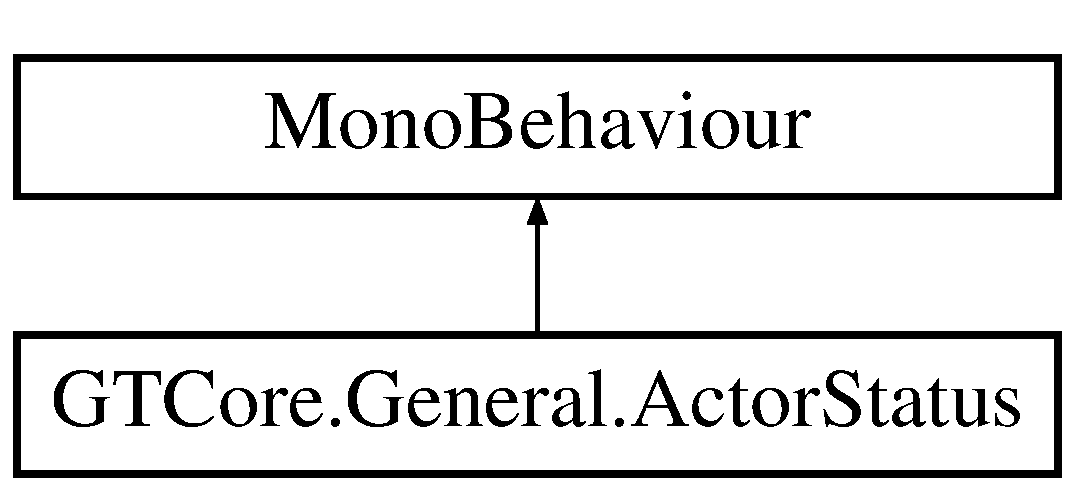
\includegraphics[height=2.000000cm]{class_g_t_core_1_1_general_1_1_actor_status}
\end{center}
\end{figure}
\subsection*{Classes}
\begin{DoxyCompactItemize}
\item 
class \hyperlink{class_g_t_core_1_1_general_1_1_actor_status_1_1_transform_storage}{Transform\+Storage}
\end{DoxyCompactItemize}
\subsection*{Public Types}
\begin{DoxyCompactItemize}
\item 
enum \hyperlink{class_g_t_core_1_1_general_1_1_actor_status_aece73cbcbe7407c6f473f67fabdca2af}{Moving\+To} \{ \\*
\hyperlink{class_g_t_core_1_1_general_1_1_actor_status_aece73cbcbe7407c6f473f67fabdca2afa6adf97f83acf6453d4a6a4b1070f3754}{Moving\+To.\+None} = (1 $<$$<$ 0), 
\hyperlink{class_g_t_core_1_1_general_1_1_actor_status_aece73cbcbe7407c6f473f67fabdca2afa258f49887ef8d14ac268c92b02503aaa}{Moving\+To.\+Up} = (1 $<$$<$ 1), 
\hyperlink{class_g_t_core_1_1_general_1_1_actor_status_aece73cbcbe7407c6f473f67fabdca2afa08a38277b0309070706f6652eeae9a53}{Moving\+To.\+Down} = (1 $<$$<$ 2), 
\hyperlink{class_g_t_core_1_1_general_1_1_actor_status_aece73cbcbe7407c6f473f67fabdca2afa945d5e233cf7d6240f6b783b36a374ff}{Moving\+To.\+Left} = (1 $<$$<$ 3), 
\\*
\hyperlink{class_g_t_core_1_1_general_1_1_actor_status_aece73cbcbe7407c6f473f67fabdca2afa92b09c7c48c520c3c55e497875da437c}{Moving\+To.\+Right} = (1 $<$$<$ 4), 
\hyperlink{class_g_t_core_1_1_general_1_1_actor_status_aece73cbcbe7407c6f473f67fabdca2afa67d2f6740a8eaebf4d5c6f79be8da481}{Moving\+To.\+Forward} = (1 $<$$<$ 5), 
\hyperlink{class_g_t_core_1_1_general_1_1_actor_status_aece73cbcbe7407c6f473f67fabdca2afa9d1104e419414f4c268be7211fb8fc4a}{Moving\+To.\+Backwards} = (1 $<$$<$ 6)
 \}
\item 
enum \hyperlink{class_g_t_core_1_1_general_1_1_actor_status_a8a2ef18692e51ef1c72e0a6478ef62e2}{Status} \{ \hyperlink{class_g_t_core_1_1_general_1_1_actor_status_a8a2ef18692e51ef1c72e0a6478ef62e2adefe967ad0373b2274fc298f19125ca7}{Status.\+Moving} = (1 $<$$<$ 0), 
\hyperlink{class_g_t_core_1_1_general_1_1_actor_status_a8a2ef18692e51ef1c72e0a6478ef62e2a52f8e1f874b075c87750fd28311b03e7}{Status.\+Turning} = (1 $<$$<$ 1), 
\hyperlink{class_g_t_core_1_1_general_1_1_actor_status_a8a2ef18692e51ef1c72e0a6478ef62e2ae599161956d626eda4cb0a5ffb85271c}{Status.\+Idle} = (1 $<$$<$ 2)
 \}
\end{DoxyCompactItemize}
\subsection*{Public Attributes}
\begin{DoxyCompactItemize}
\item 
float \hyperlink{class_g_t_core_1_1_general_1_1_actor_status_a0a365c9c2ca1a5b136caac5d2ffd68a9}{Position\+Change\+Tolerance} = 0.\+1f
\begin{DoxyCompactList}\small\item\em \hyperlink{class_g_t_core_1_1_general_1_1_actor_status}{Actor\+Status} stores the previous position periodically, this value indicates how much the actor had to move to be considered \textquotesingle{}moving\textquotesingle{} \end{DoxyCompactList}\item 
float \hyperlink{class_g_t_core_1_1_general_1_1_actor_status_a09cf9b4d30d9694ac391b5cb692ec1da}{Refresh\+Status\+Frequency} = 0.\+25f
\begin{DoxyCompactList}\small\item\em Indicates how often the actor status will be updated, a smaller number will give the best precision \end{DoxyCompactList}\item 
float \hyperlink{class_g_t_core_1_1_general_1_1_actor_status_a38ef3887ee64950042929e342f00d015}{Turning\+Distance\+Tolerance} = 0.\+25f
\begin{DoxyCompactList}\small\item\em Every transform has three direction components up, right and forward, this value indicates how far the moving direction has to be from these vectors to consider in which direction is moving \end{DoxyCompactList}\item 
bool \hyperlink{class_g_t_core_1_1_general_1_1_actor_status_a0d0cbeef5571a70649af514bf4278069}{Use\+Square\+Distance} = false
\begin{DoxyCompactList}\small\item\em If false will use square root clasical point-\/point distance (slower) otherwise the script will use square distance \end{DoxyCompactList}\end{DoxyCompactItemize}
\subsection*{Properties}
\begin{DoxyCompactItemize}
\item 
\hyperlink{class_g_t_core_1_1_general_1_1_actor_status_a8a2ef18692e51ef1c72e0a6478ef62e2}{Status} \hyperlink{class_g_t_core_1_1_general_1_1_actor_status_a9181dd383318ffc47c661a22f1ce3ca2}{Current\+Status}\hspace{0.3cm}{\ttfamily  \mbox{[}get\mbox{]}}
\item 
\hyperlink{class_g_t_core_1_1_general_1_1_actor_status_aece73cbcbe7407c6f473f67fabdca2af}{Moving\+To} \hyperlink{class_g_t_core_1_1_general_1_1_actor_status_a8b6609e98a371dbf2918ca249ff94d78}{Move\+Direction}\hspace{0.3cm}{\ttfamily  \mbox{[}get\mbox{]}}
\end{DoxyCompactItemize}


\subsection{Detailed Description}


Definition at line 7 of file Actor\+Status.\+cs.



\subsection{Member Enumeration Documentation}
\hypertarget{class_g_t_core_1_1_general_1_1_actor_status_aece73cbcbe7407c6f473f67fabdca2af}{}\index{G\+T\+Core\+::\+General\+::\+Actor\+Status@{G\+T\+Core\+::\+General\+::\+Actor\+Status}!Moving\+To@{Moving\+To}}
\index{Moving\+To@{Moving\+To}!G\+T\+Core\+::\+General\+::\+Actor\+Status@{G\+T\+Core\+::\+General\+::\+Actor\+Status}}
\subsubsection[{Moving\+To}]{\setlength{\rightskip}{0pt plus 5cm}enum {\bf G\+T\+Core.\+General.\+Actor\+Status.\+Moving\+To}\hspace{0.3cm}{\ttfamily [strong]}}\label{class_g_t_core_1_1_general_1_1_actor_status_aece73cbcbe7407c6f473f67fabdca2af}
\begin{Desc}
\item[Enumerator]\par
\begin{description}
\index{None@{None}!G\+T\+Core\+::\+General\+::\+Actor\+Status@{G\+T\+Core\+::\+General\+::\+Actor\+Status}}\index{G\+T\+Core\+::\+General\+::\+Actor\+Status@{G\+T\+Core\+::\+General\+::\+Actor\+Status}!None@{None}}\item[{\em 
\hypertarget{class_g_t_core_1_1_general_1_1_actor_status_aece73cbcbe7407c6f473f67fabdca2afa6adf97f83acf6453d4a6a4b1070f3754}{}None\label{class_g_t_core_1_1_general_1_1_actor_status_aece73cbcbe7407c6f473f67fabdca2afa6adf97f83acf6453d4a6a4b1070f3754}
}]\index{Up@{Up}!G\+T\+Core\+::\+General\+::\+Actor\+Status@{G\+T\+Core\+::\+General\+::\+Actor\+Status}}\index{G\+T\+Core\+::\+General\+::\+Actor\+Status@{G\+T\+Core\+::\+General\+::\+Actor\+Status}!Up@{Up}}\item[{\em 
\hypertarget{class_g_t_core_1_1_general_1_1_actor_status_aece73cbcbe7407c6f473f67fabdca2afa258f49887ef8d14ac268c92b02503aaa}{}Up\label{class_g_t_core_1_1_general_1_1_actor_status_aece73cbcbe7407c6f473f67fabdca2afa258f49887ef8d14ac268c92b02503aaa}
}]\index{Down@{Down}!G\+T\+Core\+::\+General\+::\+Actor\+Status@{G\+T\+Core\+::\+General\+::\+Actor\+Status}}\index{G\+T\+Core\+::\+General\+::\+Actor\+Status@{G\+T\+Core\+::\+General\+::\+Actor\+Status}!Down@{Down}}\item[{\em 
\hypertarget{class_g_t_core_1_1_general_1_1_actor_status_aece73cbcbe7407c6f473f67fabdca2afa08a38277b0309070706f6652eeae9a53}{}Down\label{class_g_t_core_1_1_general_1_1_actor_status_aece73cbcbe7407c6f473f67fabdca2afa08a38277b0309070706f6652eeae9a53}
}]\index{Left@{Left}!G\+T\+Core\+::\+General\+::\+Actor\+Status@{G\+T\+Core\+::\+General\+::\+Actor\+Status}}\index{G\+T\+Core\+::\+General\+::\+Actor\+Status@{G\+T\+Core\+::\+General\+::\+Actor\+Status}!Left@{Left}}\item[{\em 
\hypertarget{class_g_t_core_1_1_general_1_1_actor_status_aece73cbcbe7407c6f473f67fabdca2afa945d5e233cf7d6240f6b783b36a374ff}{}Left\label{class_g_t_core_1_1_general_1_1_actor_status_aece73cbcbe7407c6f473f67fabdca2afa945d5e233cf7d6240f6b783b36a374ff}
}]\index{Right@{Right}!G\+T\+Core\+::\+General\+::\+Actor\+Status@{G\+T\+Core\+::\+General\+::\+Actor\+Status}}\index{G\+T\+Core\+::\+General\+::\+Actor\+Status@{G\+T\+Core\+::\+General\+::\+Actor\+Status}!Right@{Right}}\item[{\em 
\hypertarget{class_g_t_core_1_1_general_1_1_actor_status_aece73cbcbe7407c6f473f67fabdca2afa92b09c7c48c520c3c55e497875da437c}{}Right\label{class_g_t_core_1_1_general_1_1_actor_status_aece73cbcbe7407c6f473f67fabdca2afa92b09c7c48c520c3c55e497875da437c}
}]\index{Forward@{Forward}!G\+T\+Core\+::\+General\+::\+Actor\+Status@{G\+T\+Core\+::\+General\+::\+Actor\+Status}}\index{G\+T\+Core\+::\+General\+::\+Actor\+Status@{G\+T\+Core\+::\+General\+::\+Actor\+Status}!Forward@{Forward}}\item[{\em 
\hypertarget{class_g_t_core_1_1_general_1_1_actor_status_aece73cbcbe7407c6f473f67fabdca2afa67d2f6740a8eaebf4d5c6f79be8da481}{}Forward\label{class_g_t_core_1_1_general_1_1_actor_status_aece73cbcbe7407c6f473f67fabdca2afa67d2f6740a8eaebf4d5c6f79be8da481}
}]\index{Backwards@{Backwards}!G\+T\+Core\+::\+General\+::\+Actor\+Status@{G\+T\+Core\+::\+General\+::\+Actor\+Status}}\index{G\+T\+Core\+::\+General\+::\+Actor\+Status@{G\+T\+Core\+::\+General\+::\+Actor\+Status}!Backwards@{Backwards}}\item[{\em 
\hypertarget{class_g_t_core_1_1_general_1_1_actor_status_aece73cbcbe7407c6f473f67fabdca2afa9d1104e419414f4c268be7211fb8fc4a}{}Backwards\label{class_g_t_core_1_1_general_1_1_actor_status_aece73cbcbe7407c6f473f67fabdca2afa9d1104e419414f4c268be7211fb8fc4a}
}]\end{description}
\end{Desc}


Definition at line 12 of file Actor\+Status.\+cs.

\hypertarget{class_g_t_core_1_1_general_1_1_actor_status_a8a2ef18692e51ef1c72e0a6478ef62e2}{}\index{G\+T\+Core\+::\+General\+::\+Actor\+Status@{G\+T\+Core\+::\+General\+::\+Actor\+Status}!Status@{Status}}
\index{Status@{Status}!G\+T\+Core\+::\+General\+::\+Actor\+Status@{G\+T\+Core\+::\+General\+::\+Actor\+Status}}
\subsubsection[{Status}]{\setlength{\rightskip}{0pt plus 5cm}enum {\bf G\+T\+Core.\+General.\+Actor\+Status.\+Status}\hspace{0.3cm}{\ttfamily [strong]}}\label{class_g_t_core_1_1_general_1_1_actor_status_a8a2ef18692e51ef1c72e0a6478ef62e2}
\begin{Desc}
\item[Enumerator]\par
\begin{description}
\index{Moving@{Moving}!G\+T\+Core\+::\+General\+::\+Actor\+Status@{G\+T\+Core\+::\+General\+::\+Actor\+Status}}\index{G\+T\+Core\+::\+General\+::\+Actor\+Status@{G\+T\+Core\+::\+General\+::\+Actor\+Status}!Moving@{Moving}}\item[{\em 
\hypertarget{class_g_t_core_1_1_general_1_1_actor_status_a8a2ef18692e51ef1c72e0a6478ef62e2adefe967ad0373b2274fc298f19125ca7}{}Moving\label{class_g_t_core_1_1_general_1_1_actor_status_a8a2ef18692e51ef1c72e0a6478ef62e2adefe967ad0373b2274fc298f19125ca7}
}]\index{Turning@{Turning}!G\+T\+Core\+::\+General\+::\+Actor\+Status@{G\+T\+Core\+::\+General\+::\+Actor\+Status}}\index{G\+T\+Core\+::\+General\+::\+Actor\+Status@{G\+T\+Core\+::\+General\+::\+Actor\+Status}!Turning@{Turning}}\item[{\em 
\hypertarget{class_g_t_core_1_1_general_1_1_actor_status_a8a2ef18692e51ef1c72e0a6478ef62e2a52f8e1f874b075c87750fd28311b03e7}{}Turning\label{class_g_t_core_1_1_general_1_1_actor_status_a8a2ef18692e51ef1c72e0a6478ef62e2a52f8e1f874b075c87750fd28311b03e7}
}]\index{Idle@{Idle}!G\+T\+Core\+::\+General\+::\+Actor\+Status@{G\+T\+Core\+::\+General\+::\+Actor\+Status}}\index{G\+T\+Core\+::\+General\+::\+Actor\+Status@{G\+T\+Core\+::\+General\+::\+Actor\+Status}!Idle@{Idle}}\item[{\em 
\hypertarget{class_g_t_core_1_1_general_1_1_actor_status_a8a2ef18692e51ef1c72e0a6478ef62e2ae599161956d626eda4cb0a5ffb85271c}{}Idle\label{class_g_t_core_1_1_general_1_1_actor_status_a8a2ef18692e51ef1c72e0a6478ef62e2ae599161956d626eda4cb0a5ffb85271c}
}]\end{description}
\end{Desc}


Definition at line 28 of file Actor\+Status.\+cs.



\subsection{Member Data Documentation}
\hypertarget{class_g_t_core_1_1_general_1_1_actor_status_a0a365c9c2ca1a5b136caac5d2ffd68a9}{}\index{G\+T\+Core\+::\+General\+::\+Actor\+Status@{G\+T\+Core\+::\+General\+::\+Actor\+Status}!Position\+Change\+Tolerance@{Position\+Change\+Tolerance}}
\index{Position\+Change\+Tolerance@{Position\+Change\+Tolerance}!G\+T\+Core\+::\+General\+::\+Actor\+Status@{G\+T\+Core\+::\+General\+::\+Actor\+Status}}
\subsubsection[{Position\+Change\+Tolerance}]{\setlength{\rightskip}{0pt plus 5cm}float G\+T\+Core.\+General.\+Actor\+Status.\+Position\+Change\+Tolerance = 0.\+1f}\label{class_g_t_core_1_1_general_1_1_actor_status_a0a365c9c2ca1a5b136caac5d2ffd68a9}


\hyperlink{class_g_t_core_1_1_general_1_1_actor_status}{Actor\+Status} stores the previous position periodically, this value indicates how much the actor had to move to be considered \textquotesingle{}moving\textquotesingle{} 



Definition at line 58 of file Actor\+Status.\+cs.

\hypertarget{class_g_t_core_1_1_general_1_1_actor_status_a09cf9b4d30d9694ac391b5cb692ec1da}{}\index{G\+T\+Core\+::\+General\+::\+Actor\+Status@{G\+T\+Core\+::\+General\+::\+Actor\+Status}!Refresh\+Status\+Frequency@{Refresh\+Status\+Frequency}}
\index{Refresh\+Status\+Frequency@{Refresh\+Status\+Frequency}!G\+T\+Core\+::\+General\+::\+Actor\+Status@{G\+T\+Core\+::\+General\+::\+Actor\+Status}}
\subsubsection[{Refresh\+Status\+Frequency}]{\setlength{\rightskip}{0pt plus 5cm}float G\+T\+Core.\+General.\+Actor\+Status.\+Refresh\+Status\+Frequency = 0.\+25f}\label{class_g_t_core_1_1_general_1_1_actor_status_a09cf9b4d30d9694ac391b5cb692ec1da}


Indicates how often the actor status will be updated, a smaller number will give the best precision 



Definition at line 65 of file Actor\+Status.\+cs.

\hypertarget{class_g_t_core_1_1_general_1_1_actor_status_a38ef3887ee64950042929e342f00d015}{}\index{G\+T\+Core\+::\+General\+::\+Actor\+Status@{G\+T\+Core\+::\+General\+::\+Actor\+Status}!Turning\+Distance\+Tolerance@{Turning\+Distance\+Tolerance}}
\index{Turning\+Distance\+Tolerance@{Turning\+Distance\+Tolerance}!G\+T\+Core\+::\+General\+::\+Actor\+Status@{G\+T\+Core\+::\+General\+::\+Actor\+Status}}
\subsubsection[{Turning\+Distance\+Tolerance}]{\setlength{\rightskip}{0pt plus 5cm}float G\+T\+Core.\+General.\+Actor\+Status.\+Turning\+Distance\+Tolerance = 0.\+25f}\label{class_g_t_core_1_1_general_1_1_actor_status_a38ef3887ee64950042929e342f00d015}


Every transform has three direction components up, right and forward, this value indicates how far the moving direction has to be from these vectors to consider in which direction is moving 



Definition at line 73 of file Actor\+Status.\+cs.

\hypertarget{class_g_t_core_1_1_general_1_1_actor_status_a0d0cbeef5571a70649af514bf4278069}{}\index{G\+T\+Core\+::\+General\+::\+Actor\+Status@{G\+T\+Core\+::\+General\+::\+Actor\+Status}!Use\+Square\+Distance@{Use\+Square\+Distance}}
\index{Use\+Square\+Distance@{Use\+Square\+Distance}!G\+T\+Core\+::\+General\+::\+Actor\+Status@{G\+T\+Core\+::\+General\+::\+Actor\+Status}}
\subsubsection[{Use\+Square\+Distance}]{\setlength{\rightskip}{0pt plus 5cm}bool G\+T\+Core.\+General.\+Actor\+Status.\+Use\+Square\+Distance = false}\label{class_g_t_core_1_1_general_1_1_actor_status_a0d0cbeef5571a70649af514bf4278069}


If false will use square root clasical point-\/point distance (slower) otherwise the script will use square distance 



Definition at line 80 of file Actor\+Status.\+cs.



\subsection{Property Documentation}
\hypertarget{class_g_t_core_1_1_general_1_1_actor_status_a9181dd383318ffc47c661a22f1ce3ca2}{}\index{G\+T\+Core\+::\+General\+::\+Actor\+Status@{G\+T\+Core\+::\+General\+::\+Actor\+Status}!Current\+Status@{Current\+Status}}
\index{Current\+Status@{Current\+Status}!G\+T\+Core\+::\+General\+::\+Actor\+Status@{G\+T\+Core\+::\+General\+::\+Actor\+Status}}
\subsubsection[{Current\+Status}]{\setlength{\rightskip}{0pt plus 5cm}{\bf Status} G\+T\+Core.\+General.\+Actor\+Status.\+Current\+Status\hspace{0.3cm}{\ttfamily [get]}}\label{class_g_t_core_1_1_general_1_1_actor_status_a9181dd383318ffc47c661a22f1ce3ca2}


Definition at line 83 of file Actor\+Status.\+cs.

\hypertarget{class_g_t_core_1_1_general_1_1_actor_status_a8b6609e98a371dbf2918ca249ff94d78}{}\index{G\+T\+Core\+::\+General\+::\+Actor\+Status@{G\+T\+Core\+::\+General\+::\+Actor\+Status}!Move\+Direction@{Move\+Direction}}
\index{Move\+Direction@{Move\+Direction}!G\+T\+Core\+::\+General\+::\+Actor\+Status@{G\+T\+Core\+::\+General\+::\+Actor\+Status}}
\subsubsection[{Move\+Direction}]{\setlength{\rightskip}{0pt plus 5cm}{\bf Moving\+To} G\+T\+Core.\+General.\+Actor\+Status.\+Move\+Direction\hspace{0.3cm}{\ttfamily [get]}}\label{class_g_t_core_1_1_general_1_1_actor_status_a8b6609e98a371dbf2918ca249ff94d78}


Definition at line 89 of file Actor\+Status.\+cs.



The documentation for this class was generated from the following file\+:\begin{DoxyCompactItemize}
\item 
Assets/\+Scripts/\+G\+T\+Core/\+General/\hyperlink{_actor_status_8cs}{Actor\+Status.\+cs}\end{DoxyCompactItemize}

\hypertarget{class_g_t_utils_1_1_bit_mask_attribute}{}\section{G\+T\+Utils.\+Bit\+Mask\+Attribute Class Reference}
\label{class_g_t_utils_1_1_bit_mask_attribute}\index{G\+T\+Utils.\+Bit\+Mask\+Attribute@{G\+T\+Utils.\+Bit\+Mask\+Attribute}}
Inheritance diagram for G\+T\+Utils.\+Bit\+Mask\+Attribute\+:\begin{figure}[H]
\begin{center}
\leavevmode
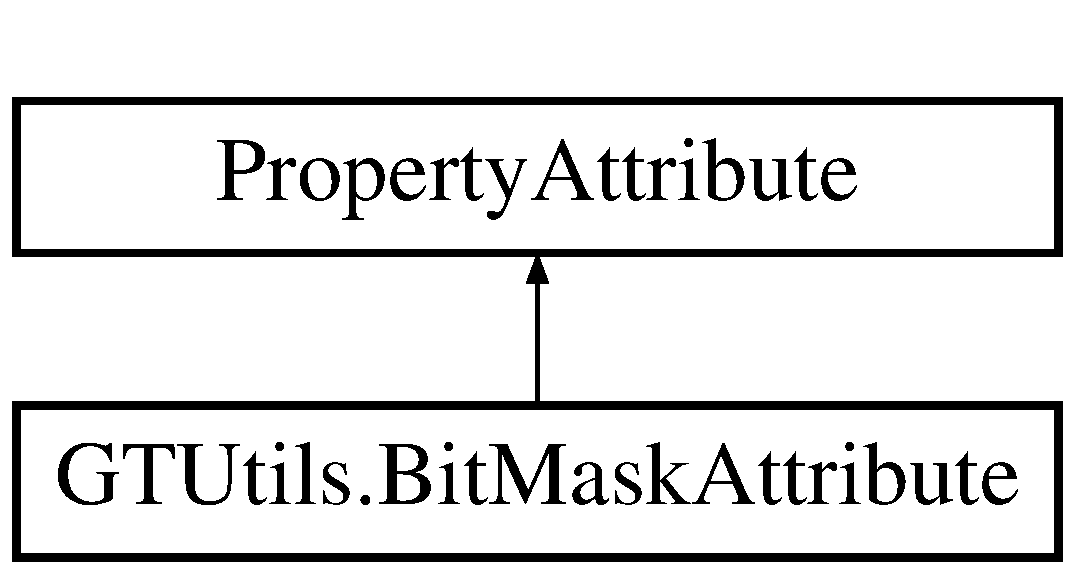
\includegraphics[height=2.000000cm]{class_g_t_utils_1_1_bit_mask_attribute}
\end{center}
\end{figure}
\subsection*{Public Member Functions}
\begin{DoxyCompactItemize}
\item 
\hyperlink{class_g_t_utils_1_1_bit_mask_attribute_a58c36d0115ac3e94ee7d8fe257ed5657}{Bit\+Mask\+Attribute} (Type a\+Type)
\end{DoxyCompactItemize}
\subsection*{Public Attributes}
\begin{DoxyCompactItemize}
\item 
Type \hyperlink{class_g_t_utils_1_1_bit_mask_attribute_aa3618cef4c4eb873925f88fe625456ad}{Prop\+Type}
\end{DoxyCompactItemize}


\subsection{Detailed Description}


Definition at line 9 of file Bit\+Mask\+Attribute.\+cs.



\subsection{Constructor \& Destructor Documentation}
\hypertarget{class_g_t_utils_1_1_bit_mask_attribute_a58c36d0115ac3e94ee7d8fe257ed5657}{}\index{G\+T\+Utils\+::\+Bit\+Mask\+Attribute@{G\+T\+Utils\+::\+Bit\+Mask\+Attribute}!Bit\+Mask\+Attribute@{Bit\+Mask\+Attribute}}
\index{Bit\+Mask\+Attribute@{Bit\+Mask\+Attribute}!G\+T\+Utils\+::\+Bit\+Mask\+Attribute@{G\+T\+Utils\+::\+Bit\+Mask\+Attribute}}
\subsubsection[{Bit\+Mask\+Attribute(\+Type a\+Type)}]{\setlength{\rightskip}{0pt plus 5cm}G\+T\+Utils.\+Bit\+Mask\+Attribute.\+Bit\+Mask\+Attribute (
\begin{DoxyParamCaption}
\item[{Type}]{a\+Type}
\end{DoxyParamCaption}
)}\label{class_g_t_utils_1_1_bit_mask_attribute_a58c36d0115ac3e94ee7d8fe257ed5657}


Definition at line 13 of file Bit\+Mask\+Attribute.\+cs.



\subsection{Member Data Documentation}
\hypertarget{class_g_t_utils_1_1_bit_mask_attribute_aa3618cef4c4eb873925f88fe625456ad}{}\index{G\+T\+Utils\+::\+Bit\+Mask\+Attribute@{G\+T\+Utils\+::\+Bit\+Mask\+Attribute}!Prop\+Type@{Prop\+Type}}
\index{Prop\+Type@{Prop\+Type}!G\+T\+Utils\+::\+Bit\+Mask\+Attribute@{G\+T\+Utils\+::\+Bit\+Mask\+Attribute}}
\subsubsection[{Prop\+Type}]{\setlength{\rightskip}{0pt plus 5cm}Type G\+T\+Utils.\+Bit\+Mask\+Attribute.\+Prop\+Type}\label{class_g_t_utils_1_1_bit_mask_attribute_aa3618cef4c4eb873925f88fe625456ad}


Definition at line 11 of file Bit\+Mask\+Attribute.\+cs.



The documentation for this class was generated from the following file\+:\begin{DoxyCompactItemize}
\item 
Assets/\+Scripts/\+G\+T\+Utils/\hyperlink{_bit_mask_attribute_8cs}{Bit\+Mask\+Attribute.\+cs}\end{DoxyCompactItemize}

\hypertarget{class_g_t_core_1_1_enviroment_1_1_bullet_parameters}{}\section{G\+T\+Core.\+Enviroment.\+Bullet\+Parameters Class Reference}
\label{class_g_t_core_1_1_enviroment_1_1_bullet_parameters}\index{G\+T\+Core.\+Enviroment.\+Bullet\+Parameters@{G\+T\+Core.\+Enviroment.\+Bullet\+Parameters}}
Inheritance diagram for G\+T\+Core.\+Enviroment.\+Bullet\+Parameters\+:\begin{figure}[H]
\begin{center}
\leavevmode
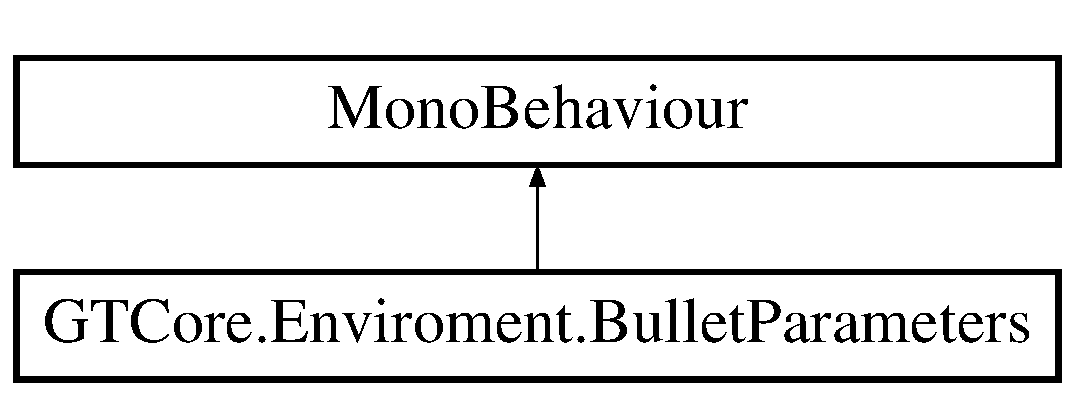
\includegraphics[height=2.000000cm]{class_g_t_core_1_1_enviroment_1_1_bullet_parameters}
\end{center}
\end{figure}
\subsection*{Public Attributes}
\begin{DoxyCompactItemize}
\item 
float \hyperlink{class_g_t_core_1_1_enviroment_1_1_bullet_parameters_a72dde58036092d5d43a50640f31e84b4}{Time\+To\+Ignore\+Owner} = 1f
\begin{DoxyCompactList}\small\item\em Bullets have an initial owner to avoid self collision \end{DoxyCompactList}\end{DoxyCompactItemize}


\subsection{Detailed Description}


Definition at line 6 of file Bullet\+Parameters.\+cs.



\subsection{Member Data Documentation}
\hypertarget{class_g_t_core_1_1_enviroment_1_1_bullet_parameters_a72dde58036092d5d43a50640f31e84b4}{}\index{G\+T\+Core\+::\+Enviroment\+::\+Bullet\+Parameters@{G\+T\+Core\+::\+Enviroment\+::\+Bullet\+Parameters}!Time\+To\+Ignore\+Owner@{Time\+To\+Ignore\+Owner}}
\index{Time\+To\+Ignore\+Owner@{Time\+To\+Ignore\+Owner}!G\+T\+Core\+::\+Enviroment\+::\+Bullet\+Parameters@{G\+T\+Core\+::\+Enviroment\+::\+Bullet\+Parameters}}
\subsubsection[{Time\+To\+Ignore\+Owner}]{\setlength{\rightskip}{0pt plus 5cm}float G\+T\+Core.\+Enviroment.\+Bullet\+Parameters.\+Time\+To\+Ignore\+Owner = 1f}\label{class_g_t_core_1_1_enviroment_1_1_bullet_parameters_a72dde58036092d5d43a50640f31e84b4}


Bullets have an initial owner to avoid self collision 



Definition at line 11 of file Bullet\+Parameters.\+cs.



The documentation for this class was generated from the following file\+:\begin{DoxyCompactItemize}
\item 
Assets/\+Scripts/\+G\+T\+Core/\+Enviroment/\hyperlink{_bullet_parameters_8cs}{Bullet\+Parameters.\+cs}\end{DoxyCompactItemize}

\hypertarget{class_g_t_core_1_1_camera_1_1_camera_movement}{}\section{G\+T\+Core.\+Camera.\+Camera\+Movement Class Reference}
\label{class_g_t_core_1_1_camera_1_1_camera_movement}\index{G\+T\+Core.\+Camera.\+Camera\+Movement@{G\+T\+Core.\+Camera.\+Camera\+Movement}}


Controls the main camera movement behaviour  


Inheritance diagram for G\+T\+Core.\+Camera.\+Camera\+Movement\+:\begin{figure}[H]
\begin{center}
\leavevmode
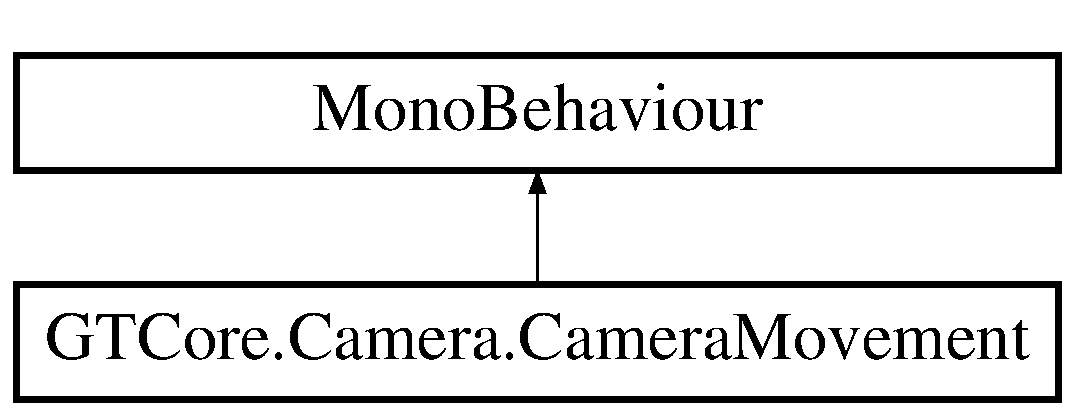
\includegraphics[height=2.000000cm]{class_g_t_core_1_1_camera_1_1_camera_movement}
\end{center}
\end{figure}
\subsection*{Public Attributes}
\begin{DoxyCompactItemize}
\item 
Vector3 \hyperlink{class_g_t_core_1_1_camera_1_1_camera_movement_a41c414edba414aada8b4a60a81dfe645}{Move\+Position} = Vector3.\+zero
\begin{DoxyCompactList}\small\item\em Moves the position of the camera relative to the target position \end{DoxyCompactList}\item 
Vector3 \hyperlink{class_g_t_core_1_1_camera_1_1_camera_movement_a6e6ee6e6693f79f8280cbd3a00787f01}{Move\+Target} = Vector3.\+zero
\begin{DoxyCompactList}\small\item\em Moves the view target position, changing the resulting direction vector \end{DoxyCompactList}\item 
float \hyperlink{class_g_t_core_1_1_camera_1_1_camera_movement_a65a4a371001a930368dc17f51c6f7b77}{Smoothing} = 5f
\begin{DoxyCompactList}\small\item\em Damps the camera movement making the movement softly reach its final position \end{DoxyCompactList}\item 
Transform \hyperlink{class_g_t_core_1_1_camera_1_1_camera_movement_a90c325f21f94e65dc0347a239bce2147}{Target}
\begin{DoxyCompactList}\small\item\em The target which the camera will be looking at \end{DoxyCompactList}\end{DoxyCompactItemize}
\subsection*{Properties}
\begin{DoxyCompactItemize}
\item 
Transform \hyperlink{class_g_t_core_1_1_camera_1_1_camera_movement_ae91326322724ddf4ef145703e4b16eba}{Non\+Interpolated\+Transform}\hspace{0.3cm}{\ttfamily  \mbox{[}get\mbox{]}}
\begin{DoxyCompactList}\small\item\em Represents the camera final position without movement smoothing \end{DoxyCompactList}\end{DoxyCompactItemize}


\subsection{Detailed Description}
Controls the main camera movement behaviour 



Definition at line 8 of file Camera\+Movement.\+cs.



\subsection{Member Data Documentation}
\hypertarget{class_g_t_core_1_1_camera_1_1_camera_movement_a41c414edba414aada8b4a60a81dfe645}{}\index{G\+T\+Core\+::\+Camera\+::\+Camera\+Movement@{G\+T\+Core\+::\+Camera\+::\+Camera\+Movement}!Move\+Position@{Move\+Position}}
\index{Move\+Position@{Move\+Position}!G\+T\+Core\+::\+Camera\+::\+Camera\+Movement@{G\+T\+Core\+::\+Camera\+::\+Camera\+Movement}}
\subsubsection[{Move\+Position}]{\setlength{\rightskip}{0pt plus 5cm}Vector3 G\+T\+Core.\+Camera.\+Camera\+Movement.\+Move\+Position = Vector3.\+zero}\label{class_g_t_core_1_1_camera_1_1_camera_movement_a41c414edba414aada8b4a60a81dfe645}


Moves the position of the camera relative to the target position 



Definition at line 14 of file Camera\+Movement.\+cs.

\hypertarget{class_g_t_core_1_1_camera_1_1_camera_movement_a6e6ee6e6693f79f8280cbd3a00787f01}{}\index{G\+T\+Core\+::\+Camera\+::\+Camera\+Movement@{G\+T\+Core\+::\+Camera\+::\+Camera\+Movement}!Move\+Target@{Move\+Target}}
\index{Move\+Target@{Move\+Target}!G\+T\+Core\+::\+Camera\+::\+Camera\+Movement@{G\+T\+Core\+::\+Camera\+::\+Camera\+Movement}}
\subsubsection[{Move\+Target}]{\setlength{\rightskip}{0pt plus 5cm}Vector3 G\+T\+Core.\+Camera.\+Camera\+Movement.\+Move\+Target = Vector3.\+zero}\label{class_g_t_core_1_1_camera_1_1_camera_movement_a6e6ee6e6693f79f8280cbd3a00787f01}


Moves the view target position, changing the resulting direction vector 



Definition at line 21 of file Camera\+Movement.\+cs.

\hypertarget{class_g_t_core_1_1_camera_1_1_camera_movement_a65a4a371001a930368dc17f51c6f7b77}{}\index{G\+T\+Core\+::\+Camera\+::\+Camera\+Movement@{G\+T\+Core\+::\+Camera\+::\+Camera\+Movement}!Smoothing@{Smoothing}}
\index{Smoothing@{Smoothing}!G\+T\+Core\+::\+Camera\+::\+Camera\+Movement@{G\+T\+Core\+::\+Camera\+::\+Camera\+Movement}}
\subsubsection[{Smoothing}]{\setlength{\rightskip}{0pt plus 5cm}float G\+T\+Core.\+Camera.\+Camera\+Movement.\+Smoothing = 5f}\label{class_g_t_core_1_1_camera_1_1_camera_movement_a65a4a371001a930368dc17f51c6f7b77}


Damps the camera movement making the movement softly reach its final position 



Definition at line 29 of file Camera\+Movement.\+cs.

\hypertarget{class_g_t_core_1_1_camera_1_1_camera_movement_a90c325f21f94e65dc0347a239bce2147}{}\index{G\+T\+Core\+::\+Camera\+::\+Camera\+Movement@{G\+T\+Core\+::\+Camera\+::\+Camera\+Movement}!Target@{Target}}
\index{Target@{Target}!G\+T\+Core\+::\+Camera\+::\+Camera\+Movement@{G\+T\+Core\+::\+Camera\+::\+Camera\+Movement}}
\subsubsection[{Target}]{\setlength{\rightskip}{0pt plus 5cm}Transform G\+T\+Core.\+Camera.\+Camera\+Movement.\+Target}\label{class_g_t_core_1_1_camera_1_1_camera_movement_a90c325f21f94e65dc0347a239bce2147}


The target which the camera will be looking at 



Definition at line 34 of file Camera\+Movement.\+cs.



\subsection{Property Documentation}
\hypertarget{class_g_t_core_1_1_camera_1_1_camera_movement_ae91326322724ddf4ef145703e4b16eba}{}\index{G\+T\+Core\+::\+Camera\+::\+Camera\+Movement@{G\+T\+Core\+::\+Camera\+::\+Camera\+Movement}!Non\+Interpolated\+Transform@{Non\+Interpolated\+Transform}}
\index{Non\+Interpolated\+Transform@{Non\+Interpolated\+Transform}!G\+T\+Core\+::\+Camera\+::\+Camera\+Movement@{G\+T\+Core\+::\+Camera\+::\+Camera\+Movement}}
\subsubsection[{Non\+Interpolated\+Transform}]{\setlength{\rightskip}{0pt plus 5cm}Transform G\+T\+Core.\+Camera.\+Camera\+Movement.\+Non\+Interpolated\+Transform\hspace{0.3cm}{\ttfamily [get]}}\label{class_g_t_core_1_1_camera_1_1_camera_movement_ae91326322724ddf4ef145703e4b16eba}


Represents the camera final position without movement smoothing 



Definition at line 39 of file Camera\+Movement.\+cs.



The documentation for this class was generated from the following file\+:\begin{DoxyCompactItemize}
\item 
Assets/\+Scripts/\+G\+T\+Core/\+Camera/\hyperlink{_camera_movement_8cs}{Camera\+Movement.\+cs}\end{DoxyCompactItemize}

\hypertarget{class_g_t_core_1_1_player_1_1_canon_movement}{}\section{G\+T\+Core.\+Player.\+Canon\+Movement Class Reference}
\label{class_g_t_core_1_1_player_1_1_canon_movement}\index{G\+T\+Core.\+Player.\+Canon\+Movement@{G\+T\+Core.\+Player.\+Canon\+Movement}}
Inheritance diagram for G\+T\+Core.\+Player.\+Canon\+Movement\+:\begin{figure}[H]
\begin{center}
\leavevmode
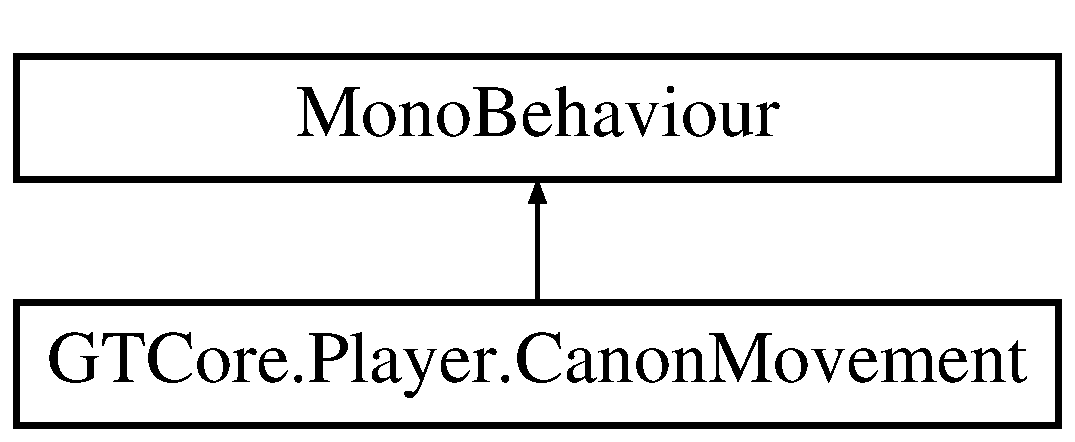
\includegraphics[height=2.000000cm]{class_g_t_core_1_1_player_1_1_canon_movement}
\end{center}
\end{figure}
\subsection*{Public Attributes}
\begin{DoxyCompactItemize}
\item 
Transform \hyperlink{class_g_t_core_1_1_player_1_1_canon_movement_af53ac38464eb96b0892af73ca9e9ed51}{Canon\+Owner}
\begin{DoxyCompactList}\small\item\em The canon will rotate around the canong owner \end{DoxyCompactList}\item 
float \hyperlink{class_g_t_core_1_1_player_1_1_canon_movement_a0fa4b6b53690e2d4b4d4e50bf108114c}{Canon\+Separation} = 0.\+5f
\begin{DoxyCompactList}\small\item\em Indicates the seperation between the canon owner and the canon \end{DoxyCompactList}\item 
float \hyperlink{class_g_t_core_1_1_player_1_1_canon_movement_ad2b5f9544754bdc5104cbb98787dbedf}{Turning\+Damping} = 8.\+0f
\begin{DoxyCompactList}\small\item\em Damps the canon rotation to make it rotate around softly \end{DoxyCompactList}\end{DoxyCompactItemize}


\subsection{Detailed Description}


Definition at line 5 of file Canon\+Movement.\+cs.



\subsection{Member Data Documentation}
\hypertarget{class_g_t_core_1_1_player_1_1_canon_movement_af53ac38464eb96b0892af73ca9e9ed51}{}\index{G\+T\+Core\+::\+Player\+::\+Canon\+Movement@{G\+T\+Core\+::\+Player\+::\+Canon\+Movement}!Canon\+Owner@{Canon\+Owner}}
\index{Canon\+Owner@{Canon\+Owner}!G\+T\+Core\+::\+Player\+::\+Canon\+Movement@{G\+T\+Core\+::\+Player\+::\+Canon\+Movement}}
\subsubsection[{Canon\+Owner}]{\setlength{\rightskip}{0pt plus 5cm}Transform G\+T\+Core.\+Player.\+Canon\+Movement.\+Canon\+Owner}\label{class_g_t_core_1_1_player_1_1_canon_movement_af53ac38464eb96b0892af73ca9e9ed51}


The canon will rotate around the canong owner 



Definition at line 12 of file Canon\+Movement.\+cs.

\hypertarget{class_g_t_core_1_1_player_1_1_canon_movement_a0fa4b6b53690e2d4b4d4e50bf108114c}{}\index{G\+T\+Core\+::\+Player\+::\+Canon\+Movement@{G\+T\+Core\+::\+Player\+::\+Canon\+Movement}!Canon\+Separation@{Canon\+Separation}}
\index{Canon\+Separation@{Canon\+Separation}!G\+T\+Core\+::\+Player\+::\+Canon\+Movement@{G\+T\+Core\+::\+Player\+::\+Canon\+Movement}}
\subsubsection[{Canon\+Separation}]{\setlength{\rightskip}{0pt plus 5cm}float G\+T\+Core.\+Player.\+Canon\+Movement.\+Canon\+Separation = 0.\+5f}\label{class_g_t_core_1_1_player_1_1_canon_movement_a0fa4b6b53690e2d4b4d4e50bf108114c}


Indicates the seperation between the canon owner and the canon 



Definition at line 18 of file Canon\+Movement.\+cs.

\hypertarget{class_g_t_core_1_1_player_1_1_canon_movement_ad2b5f9544754bdc5104cbb98787dbedf}{}\index{G\+T\+Core\+::\+Player\+::\+Canon\+Movement@{G\+T\+Core\+::\+Player\+::\+Canon\+Movement}!Turning\+Damping@{Turning\+Damping}}
\index{Turning\+Damping@{Turning\+Damping}!G\+T\+Core\+::\+Player\+::\+Canon\+Movement@{G\+T\+Core\+::\+Player\+::\+Canon\+Movement}}
\subsubsection[{Turning\+Damping}]{\setlength{\rightskip}{0pt plus 5cm}float G\+T\+Core.\+Player.\+Canon\+Movement.\+Turning\+Damping = 8.\+0f}\label{class_g_t_core_1_1_player_1_1_canon_movement_ad2b5f9544754bdc5104cbb98787dbedf}


Damps the canon rotation to make it rotate around softly 



Definition at line 24 of file Canon\+Movement.\+cs.



The documentation for this class was generated from the following file\+:\begin{DoxyCompactItemize}
\item 
Assets/\+Scripts/\+G\+T\+Core/\+Player/\hyperlink{_canon_movement_8cs}{Canon\+Movement.\+cs}\end{DoxyCompactItemize}

\hypertarget{class_enum_flags_attribute_drawer}{}\section{Enum\+Flags\+Attribute\+Drawer Class Reference}
\label{class_enum_flags_attribute_drawer}\index{Enum\+Flags\+Attribute\+Drawer@{Enum\+Flags\+Attribute\+Drawer}}
Inheritance diagram for Enum\+Flags\+Attribute\+Drawer\+:\begin{figure}[H]
\begin{center}
\leavevmode
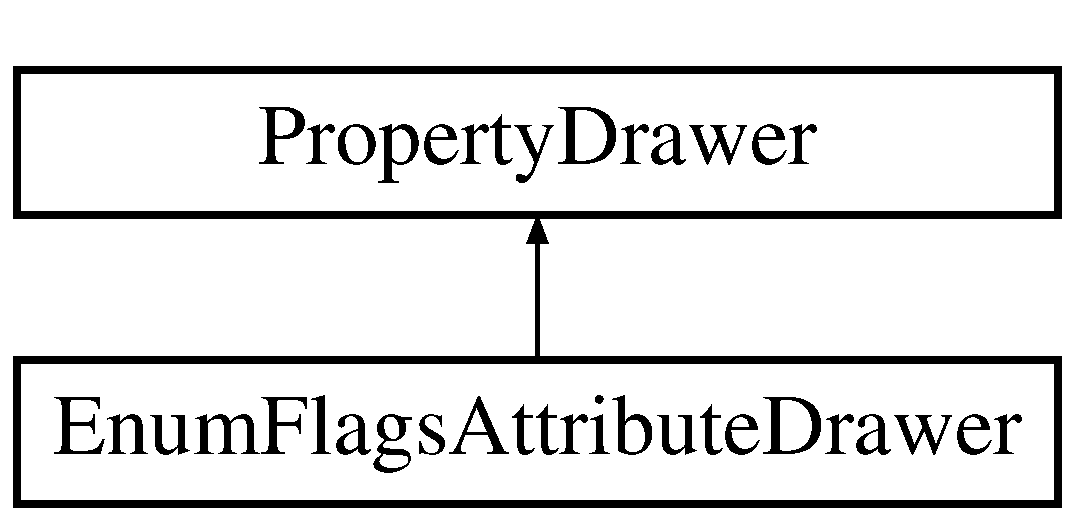
\includegraphics[height=2.000000cm]{class_enum_flags_attribute_drawer}
\end{center}
\end{figure}
\subsection*{Public Member Functions}
\begin{DoxyCompactItemize}
\item 
override void \hyperlink{class_enum_flags_attribute_drawer_a69e8be0542e3c7498871ebf2bcceb63b}{On\+G\+U\+I} (Rect position, Serialized\+Property property, G\+U\+I\+Content label)
\end{DoxyCompactItemize}


\subsection{Detailed Description}


Definition at line 8 of file Bit\+Mask\+Drawer.\+cs.



\subsection{Member Function Documentation}
\hypertarget{class_enum_flags_attribute_drawer_a69e8be0542e3c7498871ebf2bcceb63b}{}\index{Enum\+Flags\+Attribute\+Drawer@{Enum\+Flags\+Attribute\+Drawer}!On\+G\+U\+I@{On\+G\+U\+I}}
\index{On\+G\+U\+I@{On\+G\+U\+I}!Enum\+Flags\+Attribute\+Drawer@{Enum\+Flags\+Attribute\+Drawer}}
\subsubsection[{On\+G\+U\+I(\+Rect position, Serialized\+Property property, G\+U\+I\+Content label)}]{\setlength{\rightskip}{0pt plus 5cm}override void Enum\+Flags\+Attribute\+Drawer.\+On\+G\+U\+I (
\begin{DoxyParamCaption}
\item[{Rect}]{position, }
\item[{Serialized\+Property}]{property, }
\item[{G\+U\+I\+Content}]{label}
\end{DoxyParamCaption}
)}\label{class_enum_flags_attribute_drawer_a69e8be0542e3c7498871ebf2bcceb63b}


Definition at line 10 of file Bit\+Mask\+Drawer.\+cs.



The documentation for this class was generated from the following file\+:\begin{DoxyCompactItemize}
\item 
Assets/\+Editor/\hyperlink{_bit_mask_drawer_8cs}{Bit\+Mask\+Drawer.\+cs}\end{DoxyCompactItemize}

\hypertarget{class_g_t_core_1_1_enemies_1_1_follow_bomb_movement}{}\section{G\+T\+Core.\+Enemies.\+Follow\+Bomb\+Movement Class Reference}
\label{class_g_t_core_1_1_enemies_1_1_follow_bomb_movement}\index{G\+T\+Core.\+Enemies.\+Follow\+Bomb\+Movement@{G\+T\+Core.\+Enemies.\+Follow\+Bomb\+Movement}}


Defined the behaviour of the Follow\+Bomb enemy, this enemy is supposed to follow the player and explode once he is close enough or collides with the player  


Inheritance diagram for G\+T\+Core.\+Enemies.\+Follow\+Bomb\+Movement\+:\begin{figure}[H]
\begin{center}
\leavevmode
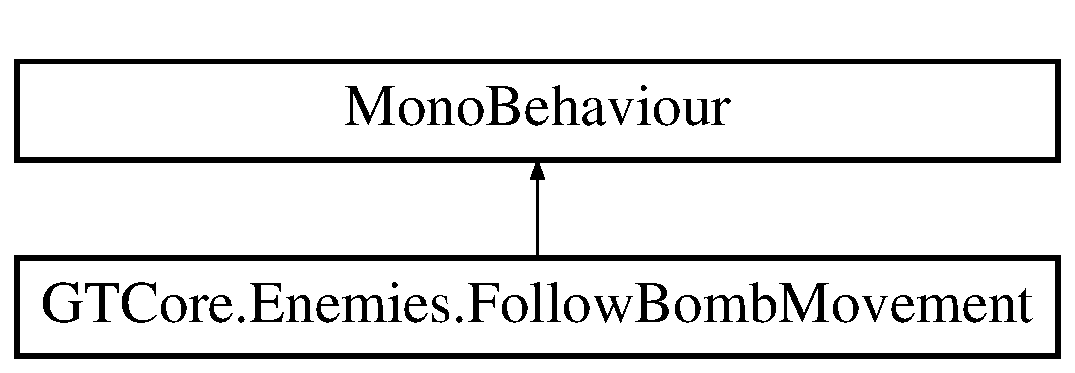
\includegraphics[height=2.000000cm]{class_g_t_core_1_1_enemies_1_1_follow_bomb_movement}
\end{center}
\end{figure}
\subsection*{Public Types}
\begin{DoxyCompactItemize}
\item 
enum \hyperlink{class_g_t_core_1_1_enemies_1_1_follow_bomb_movement_adf9532fc09595ec68cbe32713697fa48}{Movement\+Behaviour} \{ \hyperlink{class_g_t_core_1_1_enemies_1_1_follow_bomb_movement_adf9532fc09595ec68cbe32713697fa48a4457d440870ad6d42bab9082d9bf9b61}{Movement\+Behaviour.\+Fixed}, 
\hyperlink{class_g_t_core_1_1_enemies_1_1_follow_bomb_movement_adf9532fc09595ec68cbe32713697fa48acb17869fe51048b5a5c4c6106551a255}{Movement\+Behaviour.\+Constant}, 
\hyperlink{class_g_t_core_1_1_enemies_1_1_follow_bomb_movement_adf9532fc09595ec68cbe32713697fa48a9a451f1b8dbcf5ca79ee91948a53d4e0}{Movement\+Behaviour.\+Increase\+On\+Distance}, 
\hyperlink{class_g_t_core_1_1_enemies_1_1_follow_bomb_movement_adf9532fc09595ec68cbe32713697fa48a73e37c29fccdc1ddd535722e06ee00dd}{Movement\+Behaviour.\+Decrease\+On\+Distance}
 \}\begin{DoxyCompactList}\small\item\em Defines the aproaching behaviour of the follow bomb \end{DoxyCompactList}
\end{DoxyCompactItemize}
\subsection*{Public Attributes}
\begin{DoxyCompactItemize}
\item 
Vector3 \hyperlink{class_g_t_core_1_1_enemies_1_1_follow_bomb_movement_a80e25eb90a06eabb7bd3d45c2b0d8d24}{Capsule\+Begin} = Vector3.\+zero
\begin{DoxyCompactList}\small\item\em Traslates the area detection capsule beginning position from the object position, aligned with Planet center of mass \end{DoxyCompactList}\item 
Vector3 \hyperlink{class_g_t_core_1_1_enemies_1_1_follow_bomb_movement_a77d4cf25b4178b1e27b8c7251b1239db}{Capsule\+End} = Vector3.\+zero
\begin{DoxyCompactList}\small\item\em Translates the area detection capsule ending position from the object position, aligned with Planet center of mass \end{DoxyCompactList}\item 
float \hyperlink{class_g_t_core_1_1_enemies_1_1_follow_bomb_movement_aaf76d148d9b094d5a61e1412e345196f}{Capsule\+Radius} = 1f
\item 
\hyperlink{class_g_t_core_1_1_enemies_1_1_follow_bomb_movement_adf9532fc09595ec68cbe32713697fa48}{Movement\+Behaviour} \hyperlink{class_g_t_core_1_1_enemies_1_1_follow_bomb_movement_accd113a49589727e231c06b1cf02d79c}{Movement\+Type}
\item 
float \hyperlink{class_g_t_core_1_1_enemies_1_1_follow_bomb_movement_aa6e51f2d1015ecae0f9c30ce8e1c55bc}{Out\+Range\+Slowdown} = 1f
\begin{DoxyCompactList}\small\item\em Smoothing value for enemy slowdown once the player is out of range \end{DoxyCompactList}\item 
Transform \hyperlink{class_g_t_core_1_1_enemies_1_1_follow_bomb_movement_a41203fb8ac8a63c736780e054903fea8}{Planet}
\begin{DoxyCompactList}\small\item\em Planetary body where this object resides \end{DoxyCompactList}\item 
Transform \hyperlink{class_g_t_core_1_1_enemies_1_1_follow_bomb_movement_adaab5b48a877d03861e6f1e40838306e}{Player}
\item 
bool \hyperlink{class_g_t_core_1_1_enemies_1_1_follow_bomb_movement_a6acfe7e9ede561ff19f064d5f887b18b}{Use\+Square\+Distance} = false
\item 
float \hyperlink{class_g_t_core_1_1_enemies_1_1_follow_bomb_movement_a3665241c62f4b791a62f51a1e4238b8c}{Velocity\+Impulse} = 5f
\end{DoxyCompactItemize}


\subsection{Detailed Description}
Defined the behaviour of the Follow\+Bomb enemy, this enemy is supposed to follow the player and explode once he is close enough or collides with the player 



Definition at line 12 of file Follow\+Bomb\+Movement.\+cs.



\subsection{Member Enumeration Documentation}
\hypertarget{class_g_t_core_1_1_enemies_1_1_follow_bomb_movement_adf9532fc09595ec68cbe32713697fa48}{}\index{G\+T\+Core\+::\+Enemies\+::\+Follow\+Bomb\+Movement@{G\+T\+Core\+::\+Enemies\+::\+Follow\+Bomb\+Movement}!Movement\+Behaviour@{Movement\+Behaviour}}
\index{Movement\+Behaviour@{Movement\+Behaviour}!G\+T\+Core\+::\+Enemies\+::\+Follow\+Bomb\+Movement@{G\+T\+Core\+::\+Enemies\+::\+Follow\+Bomb\+Movement}}
\subsubsection[{Movement\+Behaviour}]{\setlength{\rightskip}{0pt plus 5cm}enum {\bf G\+T\+Core.\+Enemies.\+Follow\+Bomb\+Movement.\+Movement\+Behaviour}\hspace{0.3cm}{\ttfamily [strong]}}\label{class_g_t_core_1_1_enemies_1_1_follow_bomb_movement_adf9532fc09595ec68cbe32713697fa48}


Defines the aproaching behaviour of the follow bomb 

\begin{Desc}
\item[Enumerator]\par
\begin{description}
\index{Fixed@{Fixed}!G\+T\+Core\+::\+Enemies\+::\+Follow\+Bomb\+Movement@{G\+T\+Core\+::\+Enemies\+::\+Follow\+Bomb\+Movement}}\index{G\+T\+Core\+::\+Enemies\+::\+Follow\+Bomb\+Movement@{G\+T\+Core\+::\+Enemies\+::\+Follow\+Bomb\+Movement}!Fixed@{Fixed}}\item[{\em 
\hypertarget{class_g_t_core_1_1_enemies_1_1_follow_bomb_movement_adf9532fc09595ec68cbe32713697fa48a4457d440870ad6d42bab9082d9bf9b61}{}Fixed\label{class_g_t_core_1_1_enemies_1_1_follow_bomb_movement_adf9532fc09595ec68cbe32713697fa48a4457d440870ad6d42bab9082d9bf9b61}
}]\index{Constant@{Constant}!G\+T\+Core\+::\+Enemies\+::\+Follow\+Bomb\+Movement@{G\+T\+Core\+::\+Enemies\+::\+Follow\+Bomb\+Movement}}\index{G\+T\+Core\+::\+Enemies\+::\+Follow\+Bomb\+Movement@{G\+T\+Core\+::\+Enemies\+::\+Follow\+Bomb\+Movement}!Constant@{Constant}}\item[{\em 
\hypertarget{class_g_t_core_1_1_enemies_1_1_follow_bomb_movement_adf9532fc09595ec68cbe32713697fa48acb17869fe51048b5a5c4c6106551a255}{}Constant\label{class_g_t_core_1_1_enemies_1_1_follow_bomb_movement_adf9532fc09595ec68cbe32713697fa48acb17869fe51048b5a5c4c6106551a255}
}]\index{Increase\+On\+Distance@{Increase\+On\+Distance}!G\+T\+Core\+::\+Enemies\+::\+Follow\+Bomb\+Movement@{G\+T\+Core\+::\+Enemies\+::\+Follow\+Bomb\+Movement}}\index{G\+T\+Core\+::\+Enemies\+::\+Follow\+Bomb\+Movement@{G\+T\+Core\+::\+Enemies\+::\+Follow\+Bomb\+Movement}!Increase\+On\+Distance@{Increase\+On\+Distance}}\item[{\em 
\hypertarget{class_g_t_core_1_1_enemies_1_1_follow_bomb_movement_adf9532fc09595ec68cbe32713697fa48a9a451f1b8dbcf5ca79ee91948a53d4e0}{}Increase\+On\+Distance\label{class_g_t_core_1_1_enemies_1_1_follow_bomb_movement_adf9532fc09595ec68cbe32713697fa48a9a451f1b8dbcf5ca79ee91948a53d4e0}
}]\index{Decrease\+On\+Distance@{Decrease\+On\+Distance}!G\+T\+Core\+::\+Enemies\+::\+Follow\+Bomb\+Movement@{G\+T\+Core\+::\+Enemies\+::\+Follow\+Bomb\+Movement}}\index{G\+T\+Core\+::\+Enemies\+::\+Follow\+Bomb\+Movement@{G\+T\+Core\+::\+Enemies\+::\+Follow\+Bomb\+Movement}!Decrease\+On\+Distance@{Decrease\+On\+Distance}}\item[{\em 
\hypertarget{class_g_t_core_1_1_enemies_1_1_follow_bomb_movement_adf9532fc09595ec68cbe32713697fa48a73e37c29fccdc1ddd535722e06ee00dd}{}Decrease\+On\+Distance\label{class_g_t_core_1_1_enemies_1_1_follow_bomb_movement_adf9532fc09595ec68cbe32713697fa48a73e37c29fccdc1ddd535722e06ee00dd}
}]\end{description}
\end{Desc}


Definition at line 19 of file Follow\+Bomb\+Movement.\+cs.



\subsection{Member Data Documentation}
\hypertarget{class_g_t_core_1_1_enemies_1_1_follow_bomb_movement_a80e25eb90a06eabb7bd3d45c2b0d8d24}{}\index{G\+T\+Core\+::\+Enemies\+::\+Follow\+Bomb\+Movement@{G\+T\+Core\+::\+Enemies\+::\+Follow\+Bomb\+Movement}!Capsule\+Begin@{Capsule\+Begin}}
\index{Capsule\+Begin@{Capsule\+Begin}!G\+T\+Core\+::\+Enemies\+::\+Follow\+Bomb\+Movement@{G\+T\+Core\+::\+Enemies\+::\+Follow\+Bomb\+Movement}}
\subsubsection[{Capsule\+Begin}]{\setlength{\rightskip}{0pt plus 5cm}Vector3 G\+T\+Core.\+Enemies.\+Follow\+Bomb\+Movement.\+Capsule\+Begin = Vector3.\+zero}\label{class_g_t_core_1_1_enemies_1_1_follow_bomb_movement_a80e25eb90a06eabb7bd3d45c2b0d8d24}


Traslates the area detection capsule beginning position from the object position, aligned with Planet center of mass 



Definition at line 38 of file Follow\+Bomb\+Movement.\+cs.

\hypertarget{class_g_t_core_1_1_enemies_1_1_follow_bomb_movement_a77d4cf25b4178b1e27b8c7251b1239db}{}\index{G\+T\+Core\+::\+Enemies\+::\+Follow\+Bomb\+Movement@{G\+T\+Core\+::\+Enemies\+::\+Follow\+Bomb\+Movement}!Capsule\+End@{Capsule\+End}}
\index{Capsule\+End@{Capsule\+End}!G\+T\+Core\+::\+Enemies\+::\+Follow\+Bomb\+Movement@{G\+T\+Core\+::\+Enemies\+::\+Follow\+Bomb\+Movement}}
\subsubsection[{Capsule\+End}]{\setlength{\rightskip}{0pt plus 5cm}Vector3 G\+T\+Core.\+Enemies.\+Follow\+Bomb\+Movement.\+Capsule\+End = Vector3.\+zero}\label{class_g_t_core_1_1_enemies_1_1_follow_bomb_movement_a77d4cf25b4178b1e27b8c7251b1239db}


Translates the area detection capsule ending position from the object position, aligned with Planet center of mass 



Definition at line 44 of file Follow\+Bomb\+Movement.\+cs.

\hypertarget{class_g_t_core_1_1_enemies_1_1_follow_bomb_movement_aaf76d148d9b094d5a61e1412e345196f}{}\index{G\+T\+Core\+::\+Enemies\+::\+Follow\+Bomb\+Movement@{G\+T\+Core\+::\+Enemies\+::\+Follow\+Bomb\+Movement}!Capsule\+Radius@{Capsule\+Radius}}
\index{Capsule\+Radius@{Capsule\+Radius}!G\+T\+Core\+::\+Enemies\+::\+Follow\+Bomb\+Movement@{G\+T\+Core\+::\+Enemies\+::\+Follow\+Bomb\+Movement}}
\subsubsection[{Capsule\+Radius}]{\setlength{\rightskip}{0pt plus 5cm}float G\+T\+Core.\+Enemies.\+Follow\+Bomb\+Movement.\+Capsule\+Radius = 1f}\label{class_g_t_core_1_1_enemies_1_1_follow_bomb_movement_aaf76d148d9b094d5a61e1412e345196f}


Definition at line 46 of file Follow\+Bomb\+Movement.\+cs.

\hypertarget{class_g_t_core_1_1_enemies_1_1_follow_bomb_movement_accd113a49589727e231c06b1cf02d79c}{}\index{G\+T\+Core\+::\+Enemies\+::\+Follow\+Bomb\+Movement@{G\+T\+Core\+::\+Enemies\+::\+Follow\+Bomb\+Movement}!Movement\+Type@{Movement\+Type}}
\index{Movement\+Type@{Movement\+Type}!G\+T\+Core\+::\+Enemies\+::\+Follow\+Bomb\+Movement@{G\+T\+Core\+::\+Enemies\+::\+Follow\+Bomb\+Movement}}
\subsubsection[{Movement\+Type}]{\setlength{\rightskip}{0pt plus 5cm}{\bf Movement\+Behaviour} G\+T\+Core.\+Enemies.\+Follow\+Bomb\+Movement.\+Movement\+Type}\label{class_g_t_core_1_1_enemies_1_1_follow_bomb_movement_accd113a49589727e231c06b1cf02d79c}


Definition at line 47 of file Follow\+Bomb\+Movement.\+cs.

\hypertarget{class_g_t_core_1_1_enemies_1_1_follow_bomb_movement_aa6e51f2d1015ecae0f9c30ce8e1c55bc}{}\index{G\+T\+Core\+::\+Enemies\+::\+Follow\+Bomb\+Movement@{G\+T\+Core\+::\+Enemies\+::\+Follow\+Bomb\+Movement}!Out\+Range\+Slowdown@{Out\+Range\+Slowdown}}
\index{Out\+Range\+Slowdown@{Out\+Range\+Slowdown}!G\+T\+Core\+::\+Enemies\+::\+Follow\+Bomb\+Movement@{G\+T\+Core\+::\+Enemies\+::\+Follow\+Bomb\+Movement}}
\subsubsection[{Out\+Range\+Slowdown}]{\setlength{\rightskip}{0pt plus 5cm}float G\+T\+Core.\+Enemies.\+Follow\+Bomb\+Movement.\+Out\+Range\+Slowdown = 1f}\label{class_g_t_core_1_1_enemies_1_1_follow_bomb_movement_aa6e51f2d1015ecae0f9c30ce8e1c55bc}


Smoothing value for enemy slowdown once the player is out of range 



Definition at line 53 of file Follow\+Bomb\+Movement.\+cs.

\hypertarget{class_g_t_core_1_1_enemies_1_1_follow_bomb_movement_a41203fb8ac8a63c736780e054903fea8}{}\index{G\+T\+Core\+::\+Enemies\+::\+Follow\+Bomb\+Movement@{G\+T\+Core\+::\+Enemies\+::\+Follow\+Bomb\+Movement}!Planet@{Planet}}
\index{Planet@{Planet}!G\+T\+Core\+::\+Enemies\+::\+Follow\+Bomb\+Movement@{G\+T\+Core\+::\+Enemies\+::\+Follow\+Bomb\+Movement}}
\subsubsection[{Planet}]{\setlength{\rightskip}{0pt plus 5cm}Transform G\+T\+Core.\+Enemies.\+Follow\+Bomb\+Movement.\+Planet}\label{class_g_t_core_1_1_enemies_1_1_follow_bomb_movement_a41203fb8ac8a63c736780e054903fea8}


Planetary body where this object resides 



Definition at line 58 of file Follow\+Bomb\+Movement.\+cs.

\hypertarget{class_g_t_core_1_1_enemies_1_1_follow_bomb_movement_adaab5b48a877d03861e6f1e40838306e}{}\index{G\+T\+Core\+::\+Enemies\+::\+Follow\+Bomb\+Movement@{G\+T\+Core\+::\+Enemies\+::\+Follow\+Bomb\+Movement}!Player@{Player}}
\index{Player@{Player}!G\+T\+Core\+::\+Enemies\+::\+Follow\+Bomb\+Movement@{G\+T\+Core\+::\+Enemies\+::\+Follow\+Bomb\+Movement}}
\subsubsection[{Player}]{\setlength{\rightskip}{0pt plus 5cm}Transform G\+T\+Core.\+Enemies.\+Follow\+Bomb\+Movement.\+Player}\label{class_g_t_core_1_1_enemies_1_1_follow_bomb_movement_adaab5b48a877d03861e6f1e40838306e}


Definition at line 60 of file Follow\+Bomb\+Movement.\+cs.

\hypertarget{class_g_t_core_1_1_enemies_1_1_follow_bomb_movement_a6acfe7e9ede561ff19f064d5f887b18b}{}\index{G\+T\+Core\+::\+Enemies\+::\+Follow\+Bomb\+Movement@{G\+T\+Core\+::\+Enemies\+::\+Follow\+Bomb\+Movement}!Use\+Square\+Distance@{Use\+Square\+Distance}}
\index{Use\+Square\+Distance@{Use\+Square\+Distance}!G\+T\+Core\+::\+Enemies\+::\+Follow\+Bomb\+Movement@{G\+T\+Core\+::\+Enemies\+::\+Follow\+Bomb\+Movement}}
\subsubsection[{Use\+Square\+Distance}]{\setlength{\rightskip}{0pt plus 5cm}bool G\+T\+Core.\+Enemies.\+Follow\+Bomb\+Movement.\+Use\+Square\+Distance = false}\label{class_g_t_core_1_1_enemies_1_1_follow_bomb_movement_a6acfe7e9ede561ff19f064d5f887b18b}


Definition at line 61 of file Follow\+Bomb\+Movement.\+cs.

\hypertarget{class_g_t_core_1_1_enemies_1_1_follow_bomb_movement_a3665241c62f4b791a62f51a1e4238b8c}{}\index{G\+T\+Core\+::\+Enemies\+::\+Follow\+Bomb\+Movement@{G\+T\+Core\+::\+Enemies\+::\+Follow\+Bomb\+Movement}!Velocity\+Impulse@{Velocity\+Impulse}}
\index{Velocity\+Impulse@{Velocity\+Impulse}!G\+T\+Core\+::\+Enemies\+::\+Follow\+Bomb\+Movement@{G\+T\+Core\+::\+Enemies\+::\+Follow\+Bomb\+Movement}}
\subsubsection[{Velocity\+Impulse}]{\setlength{\rightskip}{0pt plus 5cm}float G\+T\+Core.\+Enemies.\+Follow\+Bomb\+Movement.\+Velocity\+Impulse = 5f}\label{class_g_t_core_1_1_enemies_1_1_follow_bomb_movement_a3665241c62f4b791a62f51a1e4238b8c}


Definition at line 62 of file Follow\+Bomb\+Movement.\+cs.



The documentation for this class was generated from the following file\+:\begin{DoxyCompactItemize}
\item 
Assets/\+Scripts/\+G\+T\+Core/\+Enemies/\hyperlink{_follow_bomb_movement_8cs}{Follow\+Bomb\+Movement.\+cs}\end{DoxyCompactItemize}

\hypertarget{class_g_t_core_1_1_enviroment_1_1_planet_info}{}\section{G\+T\+Core.\+Enviroment.\+Planet\+Info Class Reference}
\label{class_g_t_core_1_1_enviroment_1_1_planet_info}\index{G\+T\+Core.\+Enviroment.\+Planet\+Info@{G\+T\+Core.\+Enviroment.\+Planet\+Info}}
Inheritance diagram for G\+T\+Core.\+Enviroment.\+Planet\+Info\+:\begin{figure}[H]
\begin{center}
\leavevmode
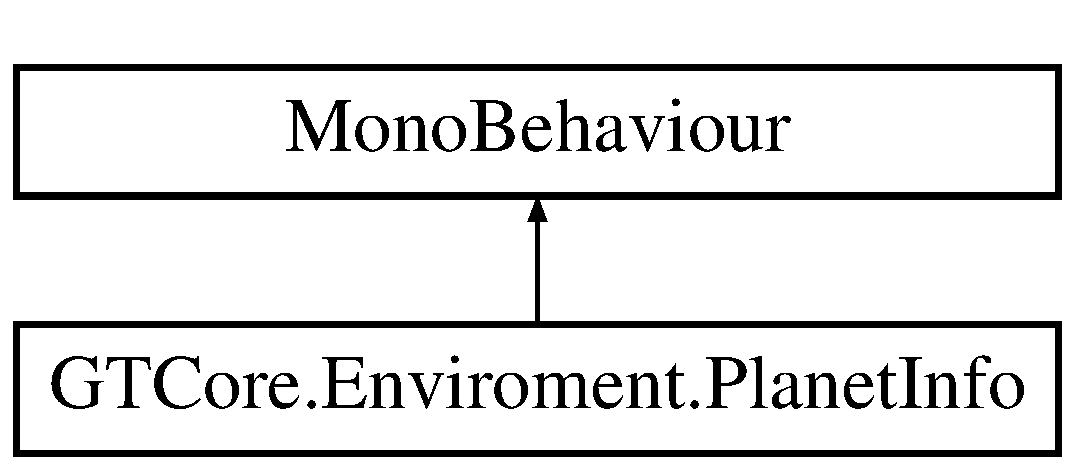
\includegraphics[height=2.000000cm]{class_g_t_core_1_1_enviroment_1_1_planet_info}
\end{center}
\end{figure}
\subsection*{Public Attributes}
\begin{DoxyCompactItemize}
\item 
float \hyperlink{class_g_t_core_1_1_enviroment_1_1_planet_info_af0fdb445b6b3bd85dd6f3147f4cd0ebd}{Gravity} = 9.\+8f
\end{DoxyCompactItemize}


\subsection{Detailed Description}


Definition at line 5 of file Planet\+Info.\+cs.



\subsection{Member Data Documentation}
\hypertarget{class_g_t_core_1_1_enviroment_1_1_planet_info_af0fdb445b6b3bd85dd6f3147f4cd0ebd}{}\index{G\+T\+Core\+::\+Enviroment\+::\+Planet\+Info@{G\+T\+Core\+::\+Enviroment\+::\+Planet\+Info}!Gravity@{Gravity}}
\index{Gravity@{Gravity}!G\+T\+Core\+::\+Enviroment\+::\+Planet\+Info@{G\+T\+Core\+::\+Enviroment\+::\+Planet\+Info}}
\subsubsection[{Gravity}]{\setlength{\rightskip}{0pt plus 5cm}float G\+T\+Core.\+Enviroment.\+Planet\+Info.\+Gravity = 9.\+8f}\label{class_g_t_core_1_1_enviroment_1_1_planet_info_af0fdb445b6b3bd85dd6f3147f4cd0ebd}


Definition at line 7 of file Planet\+Info.\+cs.



The documentation for this class was generated from the following file\+:\begin{DoxyCompactItemize}
\item 
Assets/\+Scripts/\+G\+T\+Core/\+Enviroment/\hyperlink{_planet_info_8cs}{Planet\+Info.\+cs}\end{DoxyCompactItemize}

\hypertarget{class_g_t_core_1_1_player_1_1_player_movement}{}\section{G\+T\+Core.\+Player.\+Player\+Movement Class Reference}
\label{class_g_t_core_1_1_player_1_1_player_movement}\index{G\+T\+Core.\+Player.\+Player\+Movement@{G\+T\+Core.\+Player.\+Player\+Movement}}
Inheritance diagram for G\+T\+Core.\+Player.\+Player\+Movement\+:\begin{figure}[H]
\begin{center}
\leavevmode
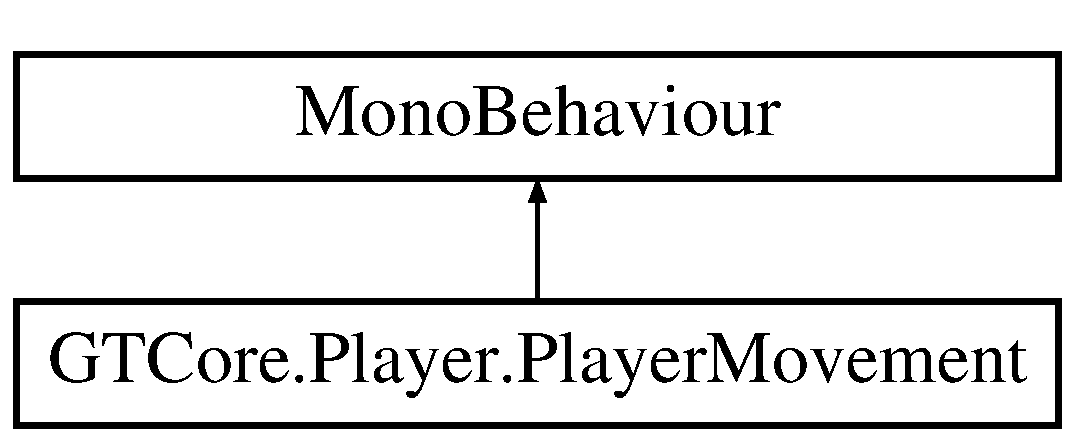
\includegraphics[height=2.000000cm]{class_g_t_core_1_1_player_1_1_player_movement}
\end{center}
\end{figure}
\subsection*{Public Attributes}
\begin{DoxyCompactItemize}
\item 
float \hyperlink{class_g_t_core_1_1_player_1_1_player_movement_a56441c76eefb5daef3c5c975d0a47e82}{Damping} = 8f
\begin{DoxyCompactList}\small\item\em Softens the player rotation / turning \end{DoxyCompactList}\item 
\hyperlink{class_g_t_core_1_1_camera_1_1_camera_movement}{Camera\+Movement} \hyperlink{class_g_t_core_1_1_player_1_1_player_movement_aeaee3024bab44f3ddef8312a2c13a31d}{Game\+Camera}
\item 
float \hyperlink{class_g_t_core_1_1_player_1_1_player_movement_acbd313912a6eda65aed7bd5a393ad1d9}{Jump\+Strength} = 2f
\item 
float \hyperlink{class_g_t_core_1_1_player_1_1_player_movement_a6b3a8ba0b37c65e7f364c6c2179b7789}{Kill\+Angular\+Velocity} = 0.\+1f
\begin{DoxyCompactList}\small\item\em Torque based solution to kill angular velocity this value decides how fast this happens \end{DoxyCompactList}\item 
float \hyperlink{class_g_t_core_1_1_player_1_1_player_movement_a37f2a584513b960296a50e17777cb491}{Movement\+Speed} = 5f
\end{DoxyCompactItemize}


\subsection{Detailed Description}


Definition at line 9 of file Player\+Movement.\+cs.



\subsection{Member Data Documentation}
\hypertarget{class_g_t_core_1_1_player_1_1_player_movement_a56441c76eefb5daef3c5c975d0a47e82}{}\index{G\+T\+Core\+::\+Player\+::\+Player\+Movement@{G\+T\+Core\+::\+Player\+::\+Player\+Movement}!Damping@{Damping}}
\index{Damping@{Damping}!G\+T\+Core\+::\+Player\+::\+Player\+Movement@{G\+T\+Core\+::\+Player\+::\+Player\+Movement}}
\subsubsection[{Damping}]{\setlength{\rightskip}{0pt plus 5cm}float G\+T\+Core.\+Player.\+Player\+Movement.\+Damping = 8f}\label{class_g_t_core_1_1_player_1_1_player_movement_a56441c76eefb5daef3c5c975d0a47e82}


Softens the player rotation / turning 



Definition at line 20 of file Player\+Movement.\+cs.

\hypertarget{class_g_t_core_1_1_player_1_1_player_movement_aeaee3024bab44f3ddef8312a2c13a31d}{}\index{G\+T\+Core\+::\+Player\+::\+Player\+Movement@{G\+T\+Core\+::\+Player\+::\+Player\+Movement}!Game\+Camera@{Game\+Camera}}
\index{Game\+Camera@{Game\+Camera}!G\+T\+Core\+::\+Player\+::\+Player\+Movement@{G\+T\+Core\+::\+Player\+::\+Player\+Movement}}
\subsubsection[{Game\+Camera}]{\setlength{\rightskip}{0pt plus 5cm}{\bf Camera\+Movement} G\+T\+Core.\+Player.\+Player\+Movement.\+Game\+Camera}\label{class_g_t_core_1_1_player_1_1_player_movement_aeaee3024bab44f3ddef8312a2c13a31d}


Definition at line 22 of file Player\+Movement.\+cs.

\hypertarget{class_g_t_core_1_1_player_1_1_player_movement_acbd313912a6eda65aed7bd5a393ad1d9}{}\index{G\+T\+Core\+::\+Player\+::\+Player\+Movement@{G\+T\+Core\+::\+Player\+::\+Player\+Movement}!Jump\+Strength@{Jump\+Strength}}
\index{Jump\+Strength@{Jump\+Strength}!G\+T\+Core\+::\+Player\+::\+Player\+Movement@{G\+T\+Core\+::\+Player\+::\+Player\+Movement}}
\subsubsection[{Jump\+Strength}]{\setlength{\rightskip}{0pt plus 5cm}float G\+T\+Core.\+Player.\+Player\+Movement.\+Jump\+Strength = 2f}\label{class_g_t_core_1_1_player_1_1_player_movement_acbd313912a6eda65aed7bd5a393ad1d9}


Definition at line 23 of file Player\+Movement.\+cs.

\hypertarget{class_g_t_core_1_1_player_1_1_player_movement_a6b3a8ba0b37c65e7f364c6c2179b7789}{}\index{G\+T\+Core\+::\+Player\+::\+Player\+Movement@{G\+T\+Core\+::\+Player\+::\+Player\+Movement}!Kill\+Angular\+Velocity@{Kill\+Angular\+Velocity}}
\index{Kill\+Angular\+Velocity@{Kill\+Angular\+Velocity}!G\+T\+Core\+::\+Player\+::\+Player\+Movement@{G\+T\+Core\+::\+Player\+::\+Player\+Movement}}
\subsubsection[{Kill\+Angular\+Velocity}]{\setlength{\rightskip}{0pt plus 5cm}float G\+T\+Core.\+Player.\+Player\+Movement.\+Kill\+Angular\+Velocity = 0.\+1f}\label{class_g_t_core_1_1_player_1_1_player_movement_a6b3a8ba0b37c65e7f364c6c2179b7789}


Torque based solution to kill angular velocity this value decides how fast this happens 



Definition at line 30 of file Player\+Movement.\+cs.

\hypertarget{class_g_t_core_1_1_player_1_1_player_movement_a37f2a584513b960296a50e17777cb491}{}\index{G\+T\+Core\+::\+Player\+::\+Player\+Movement@{G\+T\+Core\+::\+Player\+::\+Player\+Movement}!Movement\+Speed@{Movement\+Speed}}
\index{Movement\+Speed@{Movement\+Speed}!G\+T\+Core\+::\+Player\+::\+Player\+Movement@{G\+T\+Core\+::\+Player\+::\+Player\+Movement}}
\subsubsection[{Movement\+Speed}]{\setlength{\rightskip}{0pt plus 5cm}float G\+T\+Core.\+Player.\+Player\+Movement.\+Movement\+Speed = 5f}\label{class_g_t_core_1_1_player_1_1_player_movement_a37f2a584513b960296a50e17777cb491}


Definition at line 32 of file Player\+Movement.\+cs.



The documentation for this class was generated from the following file\+:\begin{DoxyCompactItemize}
\item 
Assets/\+Scripts/\+G\+T\+Core/\+Player/\hyperlink{_player_movement_8cs}{Player\+Movement.\+cs}\end{DoxyCompactItemize}

\hypertarget{class_g_t_core_1_1_player_1_1_player_shooting}{}\section{G\+T\+Core.\+Player.\+Player\+Shooting Class Reference}
\label{class_g_t_core_1_1_player_1_1_player_shooting}\index{G\+T\+Core.\+Player.\+Player\+Shooting@{G\+T\+Core.\+Player.\+Player\+Shooting}}
Inheritance diagram for G\+T\+Core.\+Player.\+Player\+Shooting\+:\begin{figure}[H]
\begin{center}
\leavevmode
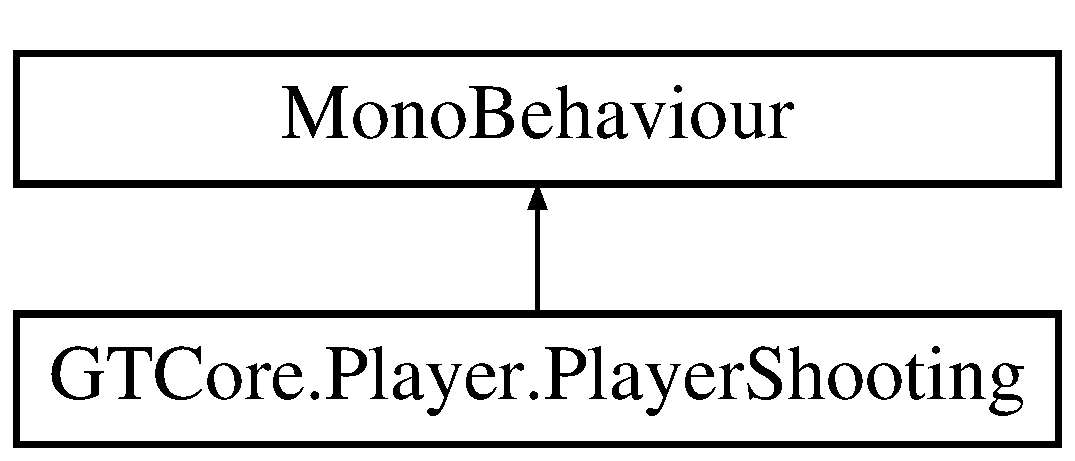
\includegraphics[height=2.000000cm]{class_g_t_core_1_1_player_1_1_player_shooting}
\end{center}
\end{figure}
\subsection*{Public Attributes}
\begin{DoxyCompactItemize}
\item 
float \hyperlink{class_g_t_core_1_1_player_1_1_player_shooting_a155b801d0290db5d7f22570912a391ba}{Bullet\+Life\+Time} = 2f
\item 
Game\+Object \hyperlink{class_g_t_core_1_1_player_1_1_player_shooting_a51b4f43ad1484327b923fd5ee6aa3e88}{Bullet\+Object}
\item 
float \hyperlink{class_g_t_core_1_1_player_1_1_player_shooting_a4666947a39a68d315e612c4b8fd27804}{Bullet\+Speed} = 5f
\end{DoxyCompactItemize}


\subsection{Detailed Description}


Definition at line 5 of file Player\+Shooting.\+cs.



\subsection{Member Data Documentation}
\hypertarget{class_g_t_core_1_1_player_1_1_player_shooting_a155b801d0290db5d7f22570912a391ba}{}\index{G\+T\+Core\+::\+Player\+::\+Player\+Shooting@{G\+T\+Core\+::\+Player\+::\+Player\+Shooting}!Bullet\+Life\+Time@{Bullet\+Life\+Time}}
\index{Bullet\+Life\+Time@{Bullet\+Life\+Time}!G\+T\+Core\+::\+Player\+::\+Player\+Shooting@{G\+T\+Core\+::\+Player\+::\+Player\+Shooting}}
\subsubsection[{Bullet\+Life\+Time}]{\setlength{\rightskip}{0pt plus 5cm}float G\+T\+Core.\+Player.\+Player\+Shooting.\+Bullet\+Life\+Time = 2f}\label{class_g_t_core_1_1_player_1_1_player_shooting_a155b801d0290db5d7f22570912a391ba}


Definition at line 7 of file Player\+Shooting.\+cs.

\hypertarget{class_g_t_core_1_1_player_1_1_player_shooting_a51b4f43ad1484327b923fd5ee6aa3e88}{}\index{G\+T\+Core\+::\+Player\+::\+Player\+Shooting@{G\+T\+Core\+::\+Player\+::\+Player\+Shooting}!Bullet\+Object@{Bullet\+Object}}
\index{Bullet\+Object@{Bullet\+Object}!G\+T\+Core\+::\+Player\+::\+Player\+Shooting@{G\+T\+Core\+::\+Player\+::\+Player\+Shooting}}
\subsubsection[{Bullet\+Object}]{\setlength{\rightskip}{0pt plus 5cm}Game\+Object G\+T\+Core.\+Player.\+Player\+Shooting.\+Bullet\+Object}\label{class_g_t_core_1_1_player_1_1_player_shooting_a51b4f43ad1484327b923fd5ee6aa3e88}


Definition at line 8 of file Player\+Shooting.\+cs.

\hypertarget{class_g_t_core_1_1_player_1_1_player_shooting_a4666947a39a68d315e612c4b8fd27804}{}\index{G\+T\+Core\+::\+Player\+::\+Player\+Shooting@{G\+T\+Core\+::\+Player\+::\+Player\+Shooting}!Bullet\+Speed@{Bullet\+Speed}}
\index{Bullet\+Speed@{Bullet\+Speed}!G\+T\+Core\+::\+Player\+::\+Player\+Shooting@{G\+T\+Core\+::\+Player\+::\+Player\+Shooting}}
\subsubsection[{Bullet\+Speed}]{\setlength{\rightskip}{0pt plus 5cm}float G\+T\+Core.\+Player.\+Player\+Shooting.\+Bullet\+Speed = 5f}\label{class_g_t_core_1_1_player_1_1_player_shooting_a4666947a39a68d315e612c4b8fd27804}


Definition at line 9 of file Player\+Shooting.\+cs.



The documentation for this class was generated from the following file\+:\begin{DoxyCompactItemize}
\item 
Assets/\+Scripts/\+G\+T\+Core/\+Player/\hyperlink{_player_shooting_8cs}{Player\+Shooting.\+cs}\end{DoxyCompactItemize}

\hypertarget{class_g_t_core_1_1_enviroment_1_1_satellite_movement}{}\section{G\+T\+Core.\+Enviroment.\+Satellite\+Movement Class Reference}
\label{class_g_t_core_1_1_enviroment_1_1_satellite_movement}\index{G\+T\+Core.\+Enviroment.\+Satellite\+Movement@{G\+T\+Core.\+Enviroment.\+Satellite\+Movement}}
Inheritance diagram for G\+T\+Core.\+Enviroment.\+Satellite\+Movement\+:\begin{figure}[H]
\begin{center}
\leavevmode
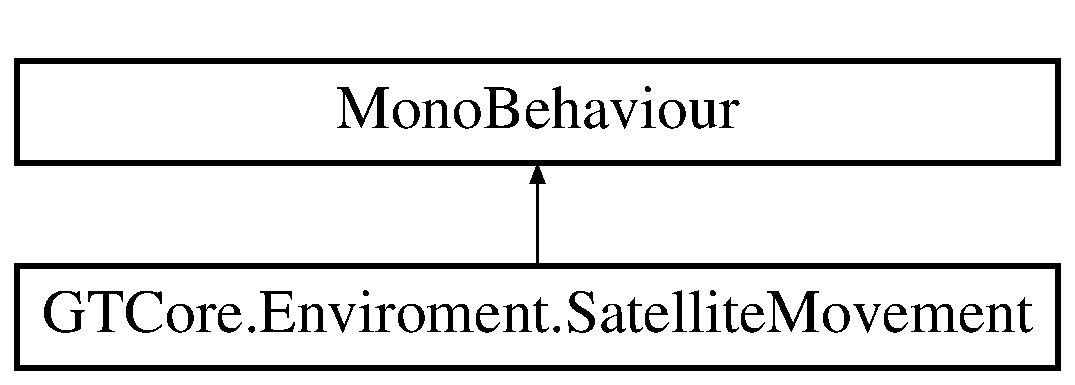
\includegraphics[height=2.000000cm]{class_g_t_core_1_1_enviroment_1_1_satellite_movement}
\end{center}
\end{figure}
\subsection*{Public Attributes}
\begin{DoxyCompactItemize}
\item 
uint \hyperlink{class_g_t_core_1_1_enviroment_1_1_satellite_movement_a4367ff0305eef42e5f23cdd3dcee1d6b}{Curve\+Precision} = 100
\begin{DoxyCompactList}\small\item\em Precision of the final point list, higher = less points \end{DoxyCompactList}\item 
float \hyperlink{class_g_t_core_1_1_enviroment_1_1_satellite_movement_a2bcfe4e72d44e5c6850f151bea94ff0d}{Distance\+Time\+Step} = 0.\+02f
\begin{DoxyCompactList}\small\item\em Distance $\ast$ Time simulation step through orbit, higher = less points \end{DoxyCompactList}\item 
List$<$ \hyperlink{class_g_t_core_1_1_enviroment_1_1_spherical_gravity}{Spherical\+Gravity} $>$ \hyperlink{class_g_t_core_1_1_enviroment_1_1_satellite_movement_a584e1245a9f119598f6fec5556612484}{Gravity\+Objects}
\begin{DoxyCompactList}\small\item\em Gravitational bodies which this object interacts with \end{DoxyCompactList}\item 
int \hyperlink{class_g_t_core_1_1_enviroment_1_1_satellite_movement_af7c8eb740e4d9802edadfa1d4c605f26}{Max\+Simulation\+Count} = 10000
\begin{DoxyCompactList}\small\item\em Maximum number of points to simulate orbit, important to stop long simulations \end{DoxyCompactList}\item 
float \hyperlink{class_g_t_core_1_1_enviroment_1_1_satellite_movement_a50b66bcd0969474ef47af91dcd129b72}{Orbital\+Speed\+Factor} = 1f
\begin{DoxyCompactList}\small\item\em Controls the speed in which the object complets its orbit \end{DoxyCompactList}\item 
float \hyperlink{class_g_t_core_1_1_enviroment_1_1_satellite_movement_a87d2eb7380cf22cc86c30e8812eabe28}{Orbit\+Tolerance\+Distance} = 0.\+05f
\begin{DoxyCompactList}\small\item\em Distance of the last point to the first point on orbit to be considered stable \end{DoxyCompactList}\item 
Vector3 \hyperlink{class_g_t_core_1_1_enviroment_1_1_satellite_movement_a40de5e52bf15f802fc963ff3ee3434bc}{Starting\+Velocity} = Vector3.\+up
\end{DoxyCompactItemize}


\subsection{Detailed Description}


Definition at line 10 of file Satellite\+Movement.\+cs.



\subsection{Member Data Documentation}
\hypertarget{class_g_t_core_1_1_enviroment_1_1_satellite_movement_a4367ff0305eef42e5f23cdd3dcee1d6b}{}\index{G\+T\+Core\+::\+Enviroment\+::\+Satellite\+Movement@{G\+T\+Core\+::\+Enviroment\+::\+Satellite\+Movement}!Curve\+Precision@{Curve\+Precision}}
\index{Curve\+Precision@{Curve\+Precision}!G\+T\+Core\+::\+Enviroment\+::\+Satellite\+Movement@{G\+T\+Core\+::\+Enviroment\+::\+Satellite\+Movement}}
\subsubsection[{Curve\+Precision}]{\setlength{\rightskip}{0pt plus 5cm}uint G\+T\+Core.\+Enviroment.\+Satellite\+Movement.\+Curve\+Precision = 100}\label{class_g_t_core_1_1_enviroment_1_1_satellite_movement_a4367ff0305eef42e5f23cdd3dcee1d6b}


Precision of the final point list, higher = less points 



Definition at line 25 of file Satellite\+Movement.\+cs.

\hypertarget{class_g_t_core_1_1_enviroment_1_1_satellite_movement_a2bcfe4e72d44e5c6850f151bea94ff0d}{}\index{G\+T\+Core\+::\+Enviroment\+::\+Satellite\+Movement@{G\+T\+Core\+::\+Enviroment\+::\+Satellite\+Movement}!Distance\+Time\+Step@{Distance\+Time\+Step}}
\index{Distance\+Time\+Step@{Distance\+Time\+Step}!G\+T\+Core\+::\+Enviroment\+::\+Satellite\+Movement@{G\+T\+Core\+::\+Enviroment\+::\+Satellite\+Movement}}
\subsubsection[{Distance\+Time\+Step}]{\setlength{\rightskip}{0pt plus 5cm}float G\+T\+Core.\+Enviroment.\+Satellite\+Movement.\+Distance\+Time\+Step = 0.\+02f}\label{class_g_t_core_1_1_enviroment_1_1_satellite_movement_a2bcfe4e72d44e5c6850f151bea94ff0d}


Distance $\ast$ Time simulation step through orbit, higher = less points 



Definition at line 32 of file Satellite\+Movement.\+cs.

\hypertarget{class_g_t_core_1_1_enviroment_1_1_satellite_movement_a584e1245a9f119598f6fec5556612484}{}\index{G\+T\+Core\+::\+Enviroment\+::\+Satellite\+Movement@{G\+T\+Core\+::\+Enviroment\+::\+Satellite\+Movement}!Gravity\+Objects@{Gravity\+Objects}}
\index{Gravity\+Objects@{Gravity\+Objects}!G\+T\+Core\+::\+Enviroment\+::\+Satellite\+Movement@{G\+T\+Core\+::\+Enviroment\+::\+Satellite\+Movement}}
\subsubsection[{Gravity\+Objects}]{\setlength{\rightskip}{0pt plus 5cm}List$<${\bf Spherical\+Gravity}$>$ G\+T\+Core.\+Enviroment.\+Satellite\+Movement.\+Gravity\+Objects}\label{class_g_t_core_1_1_enviroment_1_1_satellite_movement_a584e1245a9f119598f6fec5556612484}


Gravitational bodies which this object interacts with 



Definition at line 38 of file Satellite\+Movement.\+cs.

\hypertarget{class_g_t_core_1_1_enviroment_1_1_satellite_movement_af7c8eb740e4d9802edadfa1d4c605f26}{}\index{G\+T\+Core\+::\+Enviroment\+::\+Satellite\+Movement@{G\+T\+Core\+::\+Enviroment\+::\+Satellite\+Movement}!Max\+Simulation\+Count@{Max\+Simulation\+Count}}
\index{Max\+Simulation\+Count@{Max\+Simulation\+Count}!G\+T\+Core\+::\+Enviroment\+::\+Satellite\+Movement@{G\+T\+Core\+::\+Enviroment\+::\+Satellite\+Movement}}
\subsubsection[{Max\+Simulation\+Count}]{\setlength{\rightskip}{0pt plus 5cm}int G\+T\+Core.\+Enviroment.\+Satellite\+Movement.\+Max\+Simulation\+Count = 10000}\label{class_g_t_core_1_1_enviroment_1_1_satellite_movement_af7c8eb740e4d9802edadfa1d4c605f26}


Maximum number of points to simulate orbit, important to stop long simulations 



Definition at line 45 of file Satellite\+Movement.\+cs.

\hypertarget{class_g_t_core_1_1_enviroment_1_1_satellite_movement_a50b66bcd0969474ef47af91dcd129b72}{}\index{G\+T\+Core\+::\+Enviroment\+::\+Satellite\+Movement@{G\+T\+Core\+::\+Enviroment\+::\+Satellite\+Movement}!Orbital\+Speed\+Factor@{Orbital\+Speed\+Factor}}
\index{Orbital\+Speed\+Factor@{Orbital\+Speed\+Factor}!G\+T\+Core\+::\+Enviroment\+::\+Satellite\+Movement@{G\+T\+Core\+::\+Enviroment\+::\+Satellite\+Movement}}
\subsubsection[{Orbital\+Speed\+Factor}]{\setlength{\rightskip}{0pt plus 5cm}float G\+T\+Core.\+Enviroment.\+Satellite\+Movement.\+Orbital\+Speed\+Factor = 1f}\label{class_g_t_core_1_1_enviroment_1_1_satellite_movement_a50b66bcd0969474ef47af91dcd129b72}


Controls the speed in which the object complets its orbit 



Definition at line 51 of file Satellite\+Movement.\+cs.

\hypertarget{class_g_t_core_1_1_enviroment_1_1_satellite_movement_a87d2eb7380cf22cc86c30e8812eabe28}{}\index{G\+T\+Core\+::\+Enviroment\+::\+Satellite\+Movement@{G\+T\+Core\+::\+Enviroment\+::\+Satellite\+Movement}!Orbit\+Tolerance\+Distance@{Orbit\+Tolerance\+Distance}}
\index{Orbit\+Tolerance\+Distance@{Orbit\+Tolerance\+Distance}!G\+T\+Core\+::\+Enviroment\+::\+Satellite\+Movement@{G\+T\+Core\+::\+Enviroment\+::\+Satellite\+Movement}}
\subsubsection[{Orbit\+Tolerance\+Distance}]{\setlength{\rightskip}{0pt plus 5cm}float G\+T\+Core.\+Enviroment.\+Satellite\+Movement.\+Orbit\+Tolerance\+Distance = 0.\+05f}\label{class_g_t_core_1_1_enviroment_1_1_satellite_movement_a87d2eb7380cf22cc86c30e8812eabe28}


Distance of the last point to the first point on orbit to be considered stable 



Definition at line 58 of file Satellite\+Movement.\+cs.

\hypertarget{class_g_t_core_1_1_enviroment_1_1_satellite_movement_a40de5e52bf15f802fc963ff3ee3434bc}{}\index{G\+T\+Core\+::\+Enviroment\+::\+Satellite\+Movement@{G\+T\+Core\+::\+Enviroment\+::\+Satellite\+Movement}!Starting\+Velocity@{Starting\+Velocity}}
\index{Starting\+Velocity@{Starting\+Velocity}!G\+T\+Core\+::\+Enviroment\+::\+Satellite\+Movement@{G\+T\+Core\+::\+Enviroment\+::\+Satellite\+Movement}}
\subsubsection[{Starting\+Velocity}]{\setlength{\rightskip}{0pt plus 5cm}Vector3 G\+T\+Core.\+Enviroment.\+Satellite\+Movement.\+Starting\+Velocity = Vector3.\+up}\label{class_g_t_core_1_1_enviroment_1_1_satellite_movement_a40de5e52bf15f802fc963ff3ee3434bc}


Definition at line 60 of file Satellite\+Movement.\+cs.



The documentation for this class was generated from the following file\+:\begin{DoxyCompactItemize}
\item 
Assets/\+Scripts/\+G\+T\+Core/\+Enviroment/\hyperlink{_satellite_movement_8cs}{Satellite\+Movement.\+cs}\end{DoxyCompactItemize}

\hypertarget{class_g_t_core_1_1_enviroment_1_1_spherical_gravity}{}\section{G\+T\+Core.\+Enviroment.\+Spherical\+Gravity Class Reference}
\label{class_g_t_core_1_1_enviroment_1_1_spherical_gravity}\index{G\+T\+Core.\+Enviroment.\+Spherical\+Gravity@{G\+T\+Core.\+Enviroment.\+Spherical\+Gravity}}
Inheritance diagram for G\+T\+Core.\+Enviroment.\+Spherical\+Gravity\+:\begin{figure}[H]
\begin{center}
\leavevmode
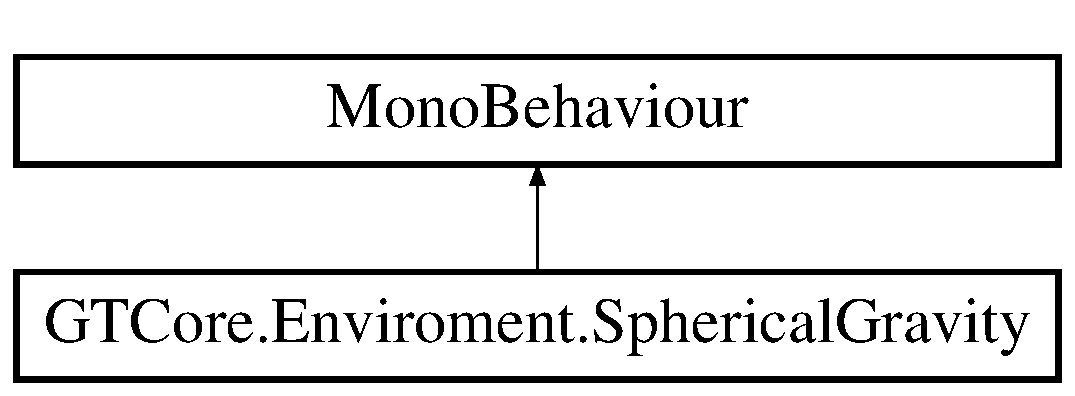
\includegraphics[height=2.000000cm]{class_g_t_core_1_1_enviroment_1_1_spherical_gravity}
\end{center}
\end{figure}
\subsection*{Public Member Functions}
\begin{DoxyCompactItemize}
\item 
Vector3 \hyperlink{class_g_t_core_1_1_enviroment_1_1_spherical_gravity_a62e4d93af1761d1303d77defa5efb849}{Get\+Center} ()
\end{DoxyCompactItemize}
\subsection*{Static Public Member Functions}
\begin{DoxyCompactItemize}
\item 
static Vector3 \hyperlink{class_g_t_core_1_1_enviroment_1_1_spherical_gravity_a4eb4a5a2cd4dff163e5ab18b787fa5a2}{Center\+Of\+Mass} (Rigidbody\mbox{[}$\,$\mbox{]} rb\+Array)
\end{DoxyCompactItemize}
\subsection*{Public Attributes}
\begin{DoxyCompactItemize}
\item 
Vector3 \hyperlink{class_g_t_core_1_1_enviroment_1_1_spherical_gravity_a1a0fdb0db303337b9ec58ca8a1ab512f}{Move\+Position} = Vector3.\+zero
\begin{DoxyCompactList}\small\item\em Moves the sphere center of mass or current center \end{DoxyCompactList}\item 
\hyperlink{class_g_t_core_1_1_enviroment_1_1_planet_info}{Planet\+Info} \hyperlink{class_g_t_core_1_1_enviroment_1_1_spherical_gravity_a1c82b6d71183bcaa8960cc83fb25912c}{Planet\+Information}
\item 
Layer\+Mask \hyperlink{class_g_t_core_1_1_enviroment_1_1_spherical_gravity_adc8b38ae5977a128be64af2f272f225c}{Pull\+Masks}
\begin{DoxyCompactList}\small\item\em Pulls the objects that reside in these masks if they posses rigidbodies \end{DoxyCompactList}\item 
float \hyperlink{class_g_t_core_1_1_enviroment_1_1_spherical_gravity_a503f1cdc6032d4bd7393fbed67af90b8}{Pull\+Radius} = 5f
\item 
bool \hyperlink{class_g_t_core_1_1_enviroment_1_1_spherical_gravity_ae3cb893e14719fe01d597926da52ab9e}{Use\+Center\+Of\+Mass} = false
\begin{DoxyCompactList}\small\item\em Enables to calculate the center of mass per update using all the rigdbodies in this transform childrens \end{DoxyCompactList}\end{DoxyCompactItemize}


\subsection{Detailed Description}


Definition at line 8 of file Spherical\+Gravity.\+cs.



\subsection{Member Function Documentation}
\hypertarget{class_g_t_core_1_1_enviroment_1_1_spherical_gravity_a4eb4a5a2cd4dff163e5ab18b787fa5a2}{}\index{G\+T\+Core\+::\+Enviroment\+::\+Spherical\+Gravity@{G\+T\+Core\+::\+Enviroment\+::\+Spherical\+Gravity}!Center\+Of\+Mass@{Center\+Of\+Mass}}
\index{Center\+Of\+Mass@{Center\+Of\+Mass}!G\+T\+Core\+::\+Enviroment\+::\+Spherical\+Gravity@{G\+T\+Core\+::\+Enviroment\+::\+Spherical\+Gravity}}
\subsubsection[{Center\+Of\+Mass(\+Rigidbody[] rb\+Array)}]{\setlength{\rightskip}{0pt plus 5cm}static Vector3 G\+T\+Core.\+Enviroment.\+Spherical\+Gravity.\+Center\+Of\+Mass (
\begin{DoxyParamCaption}
\item[{Rigidbody\mbox{[}$\,$\mbox{]}}]{rb\+Array}
\end{DoxyParamCaption}
)\hspace{0.3cm}{\ttfamily [static]}}\label{class_g_t_core_1_1_enviroment_1_1_spherical_gravity_a4eb4a5a2cd4dff163e5ab18b787fa5a2}


Definition at line 104 of file Spherical\+Gravity.\+cs.

\hypertarget{class_g_t_core_1_1_enviroment_1_1_spherical_gravity_a62e4d93af1761d1303d77defa5efb849}{}\index{G\+T\+Core\+::\+Enviroment\+::\+Spherical\+Gravity@{G\+T\+Core\+::\+Enviroment\+::\+Spherical\+Gravity}!Get\+Center@{Get\+Center}}
\index{Get\+Center@{Get\+Center}!G\+T\+Core\+::\+Enviroment\+::\+Spherical\+Gravity@{G\+T\+Core\+::\+Enviroment\+::\+Spherical\+Gravity}}
\subsubsection[{Get\+Center()}]{\setlength{\rightskip}{0pt plus 5cm}Vector3 G\+T\+Core.\+Enviroment.\+Spherical\+Gravity.\+Get\+Center (
\begin{DoxyParamCaption}
{}
\end{DoxyParamCaption}
)}\label{class_g_t_core_1_1_enviroment_1_1_spherical_gravity_a62e4d93af1761d1303d77defa5efb849}


Definition at line 50 of file Spherical\+Gravity.\+cs.



\subsection{Member Data Documentation}
\hypertarget{class_g_t_core_1_1_enviroment_1_1_spherical_gravity_a1a0fdb0db303337b9ec58ca8a1ab512f}{}\index{G\+T\+Core\+::\+Enviroment\+::\+Spherical\+Gravity@{G\+T\+Core\+::\+Enviroment\+::\+Spherical\+Gravity}!Move\+Position@{Move\+Position}}
\index{Move\+Position@{Move\+Position}!G\+T\+Core\+::\+Enviroment\+::\+Spherical\+Gravity@{G\+T\+Core\+::\+Enviroment\+::\+Spherical\+Gravity}}
\subsubsection[{Move\+Position}]{\setlength{\rightskip}{0pt plus 5cm}Vector3 G\+T\+Core.\+Enviroment.\+Spherical\+Gravity.\+Move\+Position = Vector3.\+zero}\label{class_g_t_core_1_1_enviroment_1_1_spherical_gravity_a1a0fdb0db303337b9ec58ca8a1ab512f}


Moves the sphere center of mass or current center 



Definition at line 16 of file Spherical\+Gravity.\+cs.

\hypertarget{class_g_t_core_1_1_enviroment_1_1_spherical_gravity_a1c82b6d71183bcaa8960cc83fb25912c}{}\index{G\+T\+Core\+::\+Enviroment\+::\+Spherical\+Gravity@{G\+T\+Core\+::\+Enviroment\+::\+Spherical\+Gravity}!Planet\+Information@{Planet\+Information}}
\index{Planet\+Information@{Planet\+Information}!G\+T\+Core\+::\+Enviroment\+::\+Spherical\+Gravity@{G\+T\+Core\+::\+Enviroment\+::\+Spherical\+Gravity}}
\subsubsection[{Planet\+Information}]{\setlength{\rightskip}{0pt plus 5cm}{\bf Planet\+Info} G\+T\+Core.\+Enviroment.\+Spherical\+Gravity.\+Planet\+Information}\label{class_g_t_core_1_1_enviroment_1_1_spherical_gravity_a1c82b6d71183bcaa8960cc83fb25912c}


Definition at line 18 of file Spherical\+Gravity.\+cs.

\hypertarget{class_g_t_core_1_1_enviroment_1_1_spherical_gravity_adc8b38ae5977a128be64af2f272f225c}{}\index{G\+T\+Core\+::\+Enviroment\+::\+Spherical\+Gravity@{G\+T\+Core\+::\+Enviroment\+::\+Spherical\+Gravity}!Pull\+Masks@{Pull\+Masks}}
\index{Pull\+Masks@{Pull\+Masks}!G\+T\+Core\+::\+Enviroment\+::\+Spherical\+Gravity@{G\+T\+Core\+::\+Enviroment\+::\+Spherical\+Gravity}}
\subsubsection[{Pull\+Masks}]{\setlength{\rightskip}{0pt plus 5cm}Layer\+Mask G\+T\+Core.\+Enviroment.\+Spherical\+Gravity.\+Pull\+Masks}\label{class_g_t_core_1_1_enviroment_1_1_spherical_gravity_adc8b38ae5977a128be64af2f272f225c}


Pulls the objects that reside in these masks if they posses rigidbodies 



Definition at line 25 of file Spherical\+Gravity.\+cs.

\hypertarget{class_g_t_core_1_1_enviroment_1_1_spherical_gravity_a503f1cdc6032d4bd7393fbed67af90b8}{}\index{G\+T\+Core\+::\+Enviroment\+::\+Spherical\+Gravity@{G\+T\+Core\+::\+Enviroment\+::\+Spherical\+Gravity}!Pull\+Radius@{Pull\+Radius}}
\index{Pull\+Radius@{Pull\+Radius}!G\+T\+Core\+::\+Enviroment\+::\+Spherical\+Gravity@{G\+T\+Core\+::\+Enviroment\+::\+Spherical\+Gravity}}
\subsubsection[{Pull\+Radius}]{\setlength{\rightskip}{0pt plus 5cm}float G\+T\+Core.\+Enviroment.\+Spherical\+Gravity.\+Pull\+Radius = 5f}\label{class_g_t_core_1_1_enviroment_1_1_spherical_gravity_a503f1cdc6032d4bd7393fbed67af90b8}


Definition at line 27 of file Spherical\+Gravity.\+cs.

\hypertarget{class_g_t_core_1_1_enviroment_1_1_spherical_gravity_ae3cb893e14719fe01d597926da52ab9e}{}\index{G\+T\+Core\+::\+Enviroment\+::\+Spherical\+Gravity@{G\+T\+Core\+::\+Enviroment\+::\+Spherical\+Gravity}!Use\+Center\+Of\+Mass@{Use\+Center\+Of\+Mass}}
\index{Use\+Center\+Of\+Mass@{Use\+Center\+Of\+Mass}!G\+T\+Core\+::\+Enviroment\+::\+Spherical\+Gravity@{G\+T\+Core\+::\+Enviroment\+::\+Spherical\+Gravity}}
\subsubsection[{Use\+Center\+Of\+Mass}]{\setlength{\rightskip}{0pt plus 5cm}bool G\+T\+Core.\+Enviroment.\+Spherical\+Gravity.\+Use\+Center\+Of\+Mass = false}\label{class_g_t_core_1_1_enviroment_1_1_spherical_gravity_ae3cb893e14719fe01d597926da52ab9e}


Enables to calculate the center of mass per update using all the rigdbodies in this transform childrens 



Definition at line 34 of file Spherical\+Gravity.\+cs.



The documentation for this class was generated from the following file\+:\begin{DoxyCompactItemize}
\item 
Assets/\+Scripts/\+G\+T\+Core/\+Enviroment/\hyperlink{_spherical_gravity_8cs}{Spherical\+Gravity.\+cs}\end{DoxyCompactItemize}

\hypertarget{class_g_t_core_1_1_player_1_1_stick_to_planet}{}\section{G\+T\+Core.\+Player.\+Stick\+To\+Planet Class Reference}
\label{class_g_t_core_1_1_player_1_1_stick_to_planet}\index{G\+T\+Core.\+Player.\+Stick\+To\+Planet@{G\+T\+Core.\+Player.\+Stick\+To\+Planet}}
Inheritance diagram for G\+T\+Core.\+Player.\+Stick\+To\+Planet\+:\begin{figure}[H]
\begin{center}
\leavevmode
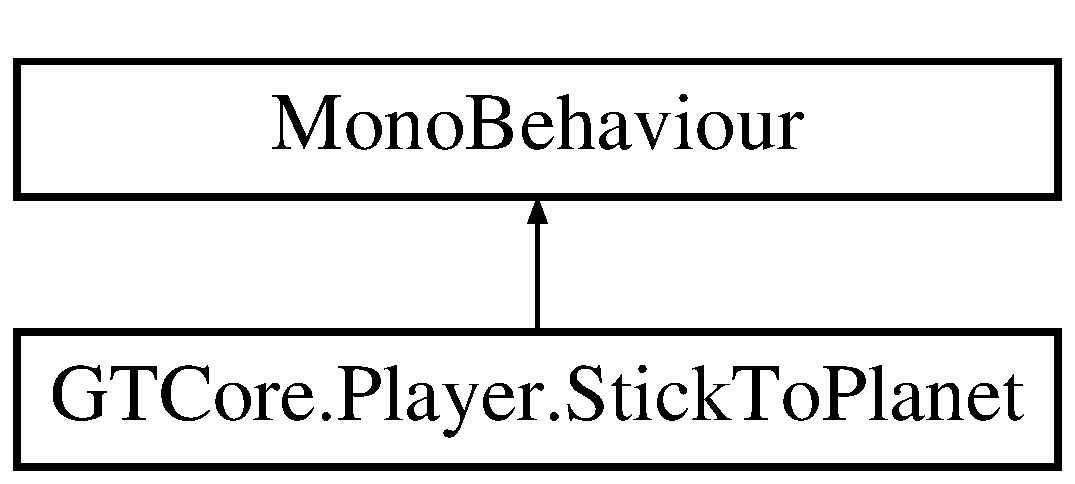
\includegraphics[height=2.000000cm]{class_g_t_core_1_1_player_1_1_stick_to_planet}
\end{center}
\end{figure}
\subsection*{Public Types}
\begin{DoxyCompactItemize}
\item 
enum \hyperlink{class_g_t_core_1_1_player_1_1_stick_to_planet_ab080d35c69764b3967026265d41fff67}{Stick\+Status} \{ \hyperlink{class_g_t_core_1_1_player_1_1_stick_to_planet_ab080d35c69764b3967026265d41fff67a0b39370ea87ef482a4def72565f537a4}{Stick\+Status.\+Stranded} = (1 $<$$<$ 0), 
\hyperlink{class_g_t_core_1_1_player_1_1_stick_to_planet_ab080d35c69764b3967026265d41fff67a2b9beed57034f5727573d7ded76cf777}{Stick\+Status.\+On\+Ground} = (1 $<$$<$ 1), 
\hyperlink{class_g_t_core_1_1_player_1_1_stick_to_planet_ab080d35c69764b3967026265d41fff67a444733081a578880ba8a563d3c59d22d}{Stick\+Status.\+Flying} = (1 $<$$<$ 2), 
\hyperlink{class_g_t_core_1_1_player_1_1_stick_to_planet_ab080d35c69764b3967026265d41fff67ad1fffb0bbc691ac077c60bd99284a005}{Stick\+Status.\+Changing\+Planet} = (1 $<$$<$ 3)
 \}
\end{DoxyCompactItemize}
\subsection*{Public Attributes}
\begin{DoxyCompactItemize}
\item 
float \hyperlink{class_g_t_core_1_1_player_1_1_stick_to_planet_abda4ff29f854ffcb71426930c1291182}{Ground\+Minimum\+Distance} = 0.\+65f
\item 
float \hyperlink{class_g_t_core_1_1_player_1_1_stick_to_planet_a88684571f58f674e9de3a305f87e4b53}{Link\+To\+Planet\+Distance} = 10f
\item 
float \hyperlink{class_g_t_core_1_1_player_1_1_stick_to_planet_a5ccaddd5d4bdc14fc1c289fca645c470}{Planet\+Change\+Damping} = 3f
\item 
\hyperlink{class_g_t_core_1_1_player_1_1_stick_to_planet_ab080d35c69764b3967026265d41fff67}{Stick\+Status} \hyperlink{class_g_t_core_1_1_player_1_1_stick_to_planet_a7fb03985d99e5effac6072d51c59811e}{Status} = \hyperlink{class_g_t_core_1_1_player_1_1_stick_to_planet_ab080d35c69764b3967026265d41fff67a0b39370ea87ef482a4def72565f537a4}{Stick\+Status.\+Stranded}
\end{DoxyCompactItemize}
\subsection*{Properties}
\begin{DoxyCompactItemize}
\item 
Vector3 \hyperlink{class_g_t_core_1_1_player_1_1_stick_to_planet_a2987fbd9ccbaba54cc7fa12b2d2d858e}{Planet\+Current\+Normal}\hspace{0.3cm}{\ttfamily  \mbox{[}get\mbox{]}}
\end{DoxyCompactItemize}


\subsection{Detailed Description}


Definition at line 9 of file Stick\+To\+Planet.\+cs.



\subsection{Member Enumeration Documentation}
\hypertarget{class_g_t_core_1_1_player_1_1_stick_to_planet_ab080d35c69764b3967026265d41fff67}{}\index{G\+T\+Core\+::\+Player\+::\+Stick\+To\+Planet@{G\+T\+Core\+::\+Player\+::\+Stick\+To\+Planet}!Stick\+Status@{Stick\+Status}}
\index{Stick\+Status@{Stick\+Status}!G\+T\+Core\+::\+Player\+::\+Stick\+To\+Planet@{G\+T\+Core\+::\+Player\+::\+Stick\+To\+Planet}}
\subsubsection[{Stick\+Status}]{\setlength{\rightskip}{0pt plus 5cm}enum {\bf G\+T\+Core.\+Player.\+Stick\+To\+Planet.\+Stick\+Status}\hspace{0.3cm}{\ttfamily [strong]}}\label{class_g_t_core_1_1_player_1_1_stick_to_planet_ab080d35c69764b3967026265d41fff67}
\begin{Desc}
\item[Enumerator]\par
\begin{description}
\index{Stranded@{Stranded}!G\+T\+Core\+::\+Player\+::\+Stick\+To\+Planet@{G\+T\+Core\+::\+Player\+::\+Stick\+To\+Planet}}\index{G\+T\+Core\+::\+Player\+::\+Stick\+To\+Planet@{G\+T\+Core\+::\+Player\+::\+Stick\+To\+Planet}!Stranded@{Stranded}}\item[{\em 
\hypertarget{class_g_t_core_1_1_player_1_1_stick_to_planet_ab080d35c69764b3967026265d41fff67a0b39370ea87ef482a4def72565f537a4}{}Stranded\label{class_g_t_core_1_1_player_1_1_stick_to_planet_ab080d35c69764b3967026265d41fff67a0b39370ea87ef482a4def72565f537a4}
}]\index{On\+Ground@{On\+Ground}!G\+T\+Core\+::\+Player\+::\+Stick\+To\+Planet@{G\+T\+Core\+::\+Player\+::\+Stick\+To\+Planet}}\index{G\+T\+Core\+::\+Player\+::\+Stick\+To\+Planet@{G\+T\+Core\+::\+Player\+::\+Stick\+To\+Planet}!On\+Ground@{On\+Ground}}\item[{\em 
\hypertarget{class_g_t_core_1_1_player_1_1_stick_to_planet_ab080d35c69764b3967026265d41fff67a2b9beed57034f5727573d7ded76cf777}{}On\+Ground\label{class_g_t_core_1_1_player_1_1_stick_to_planet_ab080d35c69764b3967026265d41fff67a2b9beed57034f5727573d7ded76cf777}
}]\index{Flying@{Flying}!G\+T\+Core\+::\+Player\+::\+Stick\+To\+Planet@{G\+T\+Core\+::\+Player\+::\+Stick\+To\+Planet}}\index{G\+T\+Core\+::\+Player\+::\+Stick\+To\+Planet@{G\+T\+Core\+::\+Player\+::\+Stick\+To\+Planet}!Flying@{Flying}}\item[{\em 
\hypertarget{class_g_t_core_1_1_player_1_1_stick_to_planet_ab080d35c69764b3967026265d41fff67a444733081a578880ba8a563d3c59d22d}{}Flying\label{class_g_t_core_1_1_player_1_1_stick_to_planet_ab080d35c69764b3967026265d41fff67a444733081a578880ba8a563d3c59d22d}
}]\index{Changing\+Planet@{Changing\+Planet}!G\+T\+Core\+::\+Player\+::\+Stick\+To\+Planet@{G\+T\+Core\+::\+Player\+::\+Stick\+To\+Planet}}\index{G\+T\+Core\+::\+Player\+::\+Stick\+To\+Planet@{G\+T\+Core\+::\+Player\+::\+Stick\+To\+Planet}!Changing\+Planet@{Changing\+Planet}}\item[{\em 
\hypertarget{class_g_t_core_1_1_player_1_1_stick_to_planet_ab080d35c69764b3967026265d41fff67ad1fffb0bbc691ac077c60bd99284a005}{}Changing\+Planet\label{class_g_t_core_1_1_player_1_1_stick_to_planet_ab080d35c69764b3967026265d41fff67ad1fffb0bbc691ac077c60bd99284a005}
}]\end{description}
\end{Desc}


Definition at line 14 of file Stick\+To\+Planet.\+cs.



\subsection{Member Data Documentation}
\hypertarget{class_g_t_core_1_1_player_1_1_stick_to_planet_abda4ff29f854ffcb71426930c1291182}{}\index{G\+T\+Core\+::\+Player\+::\+Stick\+To\+Planet@{G\+T\+Core\+::\+Player\+::\+Stick\+To\+Planet}!Ground\+Minimum\+Distance@{Ground\+Minimum\+Distance}}
\index{Ground\+Minimum\+Distance@{Ground\+Minimum\+Distance}!G\+T\+Core\+::\+Player\+::\+Stick\+To\+Planet@{G\+T\+Core\+::\+Player\+::\+Stick\+To\+Planet}}
\subsubsection[{Ground\+Minimum\+Distance}]{\setlength{\rightskip}{0pt plus 5cm}float G\+T\+Core.\+Player.\+Stick\+To\+Planet.\+Ground\+Minimum\+Distance = 0.\+65f}\label{class_g_t_core_1_1_player_1_1_stick_to_planet_abda4ff29f854ffcb71426930c1291182}


Definition at line 30 of file Stick\+To\+Planet.\+cs.

\hypertarget{class_g_t_core_1_1_player_1_1_stick_to_planet_a88684571f58f674e9de3a305f87e4b53}{}\index{G\+T\+Core\+::\+Player\+::\+Stick\+To\+Planet@{G\+T\+Core\+::\+Player\+::\+Stick\+To\+Planet}!Link\+To\+Planet\+Distance@{Link\+To\+Planet\+Distance}}
\index{Link\+To\+Planet\+Distance@{Link\+To\+Planet\+Distance}!G\+T\+Core\+::\+Player\+::\+Stick\+To\+Planet@{G\+T\+Core\+::\+Player\+::\+Stick\+To\+Planet}}
\subsubsection[{Link\+To\+Planet\+Distance}]{\setlength{\rightskip}{0pt plus 5cm}float G\+T\+Core.\+Player.\+Stick\+To\+Planet.\+Link\+To\+Planet\+Distance = 10f}\label{class_g_t_core_1_1_player_1_1_stick_to_planet_a88684571f58f674e9de3a305f87e4b53}


Definition at line 31 of file Stick\+To\+Planet.\+cs.

\hypertarget{class_g_t_core_1_1_player_1_1_stick_to_planet_a5ccaddd5d4bdc14fc1c289fca645c470}{}\index{G\+T\+Core\+::\+Player\+::\+Stick\+To\+Planet@{G\+T\+Core\+::\+Player\+::\+Stick\+To\+Planet}!Planet\+Change\+Damping@{Planet\+Change\+Damping}}
\index{Planet\+Change\+Damping@{Planet\+Change\+Damping}!G\+T\+Core\+::\+Player\+::\+Stick\+To\+Planet@{G\+T\+Core\+::\+Player\+::\+Stick\+To\+Planet}}
\subsubsection[{Planet\+Change\+Damping}]{\setlength{\rightskip}{0pt plus 5cm}float G\+T\+Core.\+Player.\+Stick\+To\+Planet.\+Planet\+Change\+Damping = 3f}\label{class_g_t_core_1_1_player_1_1_stick_to_planet_a5ccaddd5d4bdc14fc1c289fca645c470}


Definition at line 32 of file Stick\+To\+Planet.\+cs.

\hypertarget{class_g_t_core_1_1_player_1_1_stick_to_planet_a7fb03985d99e5effac6072d51c59811e}{}\index{G\+T\+Core\+::\+Player\+::\+Stick\+To\+Planet@{G\+T\+Core\+::\+Player\+::\+Stick\+To\+Planet}!Status@{Status}}
\index{Status@{Status}!G\+T\+Core\+::\+Player\+::\+Stick\+To\+Planet@{G\+T\+Core\+::\+Player\+::\+Stick\+To\+Planet}}
\subsubsection[{Status}]{\setlength{\rightskip}{0pt plus 5cm}{\bf Stick\+Status} G\+T\+Core.\+Player.\+Stick\+To\+Planet.\+Status = {\bf Stick\+Status.\+Stranded}}\label{class_g_t_core_1_1_player_1_1_stick_to_planet_a7fb03985d99e5effac6072d51c59811e}


Definition at line 35 of file Stick\+To\+Planet.\+cs.



\subsection{Property Documentation}
\hypertarget{class_g_t_core_1_1_player_1_1_stick_to_planet_a2987fbd9ccbaba54cc7fa12b2d2d858e}{}\index{G\+T\+Core\+::\+Player\+::\+Stick\+To\+Planet@{G\+T\+Core\+::\+Player\+::\+Stick\+To\+Planet}!Planet\+Current\+Normal@{Planet\+Current\+Normal}}
\index{Planet\+Current\+Normal@{Planet\+Current\+Normal}!G\+T\+Core\+::\+Player\+::\+Stick\+To\+Planet@{G\+T\+Core\+::\+Player\+::\+Stick\+To\+Planet}}
\subsubsection[{Planet\+Current\+Normal}]{\setlength{\rightskip}{0pt plus 5cm}Vector3 G\+T\+Core.\+Player.\+Stick\+To\+Planet.\+Planet\+Current\+Normal\hspace{0.3cm}{\ttfamily [get]}}\label{class_g_t_core_1_1_player_1_1_stick_to_planet_a2987fbd9ccbaba54cc7fa12b2d2d858e}


Definition at line 37 of file Stick\+To\+Planet.\+cs.



The documentation for this class was generated from the following file\+:\begin{DoxyCompactItemize}
\item 
Assets/\+Scripts/\+G\+T\+Core/\+Player/\hyperlink{_stick_to_planet_8cs}{Stick\+To\+Planet.\+cs}\end{DoxyCompactItemize}

\hypertarget{class_g_t_core_1_1_general_1_1_stick_to_player}{}\section{G\+T\+Core.\+General.\+Stick\+To\+Player Class Reference}
\label{class_g_t_core_1_1_general_1_1_stick_to_player}\index{G\+T\+Core.\+General.\+Stick\+To\+Player@{G\+T\+Core.\+General.\+Stick\+To\+Player}}
Inheritance diagram for G\+T\+Core.\+General.\+Stick\+To\+Player\+:\begin{figure}[H]
\begin{center}
\leavevmode
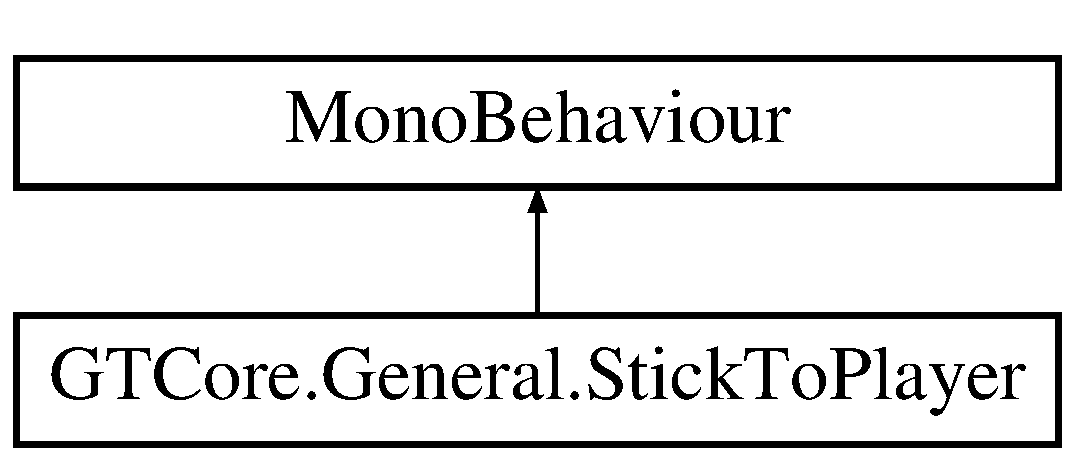
\includegraphics[height=2.000000cm]{class_g_t_core_1_1_general_1_1_stick_to_player}
\end{center}
\end{figure}
\subsection*{Public Attributes}
\begin{DoxyCompactItemize}
\item 
Transform \hyperlink{class_g_t_core_1_1_general_1_1_stick_to_player_a3a37b72f1e00a986cc40ed1be2f8da02}{Target}
\end{DoxyCompactItemize}


\subsection{Detailed Description}


Definition at line 7 of file Stick\+To\+Player.\+cs.



\subsection{Member Data Documentation}
\hypertarget{class_g_t_core_1_1_general_1_1_stick_to_player_a3a37b72f1e00a986cc40ed1be2f8da02}{}\index{G\+T\+Core\+::\+General\+::\+Stick\+To\+Player@{G\+T\+Core\+::\+General\+::\+Stick\+To\+Player}!Target@{Target}}
\index{Target@{Target}!G\+T\+Core\+::\+General\+::\+Stick\+To\+Player@{G\+T\+Core\+::\+General\+::\+Stick\+To\+Player}}
\subsubsection[{Target}]{\setlength{\rightskip}{0pt plus 5cm}Transform G\+T\+Core.\+General.\+Stick\+To\+Player.\+Target}\label{class_g_t_core_1_1_general_1_1_stick_to_player_a3a37b72f1e00a986cc40ed1be2f8da02}


Definition at line 10 of file Stick\+To\+Player.\+cs.



The documentation for this class was generated from the following file\+:\begin{DoxyCompactItemize}
\item 
Assets/\+Scripts/\+G\+T\+Core/\+General/\hyperlink{_stick_to_player_8cs}{Stick\+To\+Player.\+cs}\end{DoxyCompactItemize}

\hypertarget{class_g_t_core_1_1_general_1_1_actor_status_1_1_transform_storage}{}\section{G\+T\+Core.\+General.\+Actor\+Status.\+Transform\+Storage Class Reference}
\label{class_g_t_core_1_1_general_1_1_actor_status_1_1_transform_storage}\index{G\+T\+Core.\+General.\+Actor\+Status.\+Transform\+Storage@{G\+T\+Core.\+General.\+Actor\+Status.\+Transform\+Storage}}
\subsection*{Public Attributes}
\begin{DoxyCompactItemize}
\item 
Vector3 \hyperlink{class_g_t_core_1_1_general_1_1_actor_status_1_1_transform_storage_a45165cf14d2e4221ef59b54602494450}{Local\+Scale}
\item 
Vector3 \hyperlink{class_g_t_core_1_1_general_1_1_actor_status_1_1_transform_storage_a50f0fde9da25ebe17969c0bcc374c5f4}{Position}
\item 
Quaternion \hyperlink{class_g_t_core_1_1_general_1_1_actor_status_1_1_transform_storage_a6ad17f8ccac52b615f4124d8e3c7b09a}{Rotation}
\end{DoxyCompactItemize}


\subsection{Detailed Description}


Definition at line 191 of file Actor\+Status.\+cs.



\subsection{Member Data Documentation}
\hypertarget{class_g_t_core_1_1_general_1_1_actor_status_1_1_transform_storage_a45165cf14d2e4221ef59b54602494450}{}\index{G\+T\+Core\+::\+General\+::\+Actor\+Status\+::\+Transform\+Storage@{G\+T\+Core\+::\+General\+::\+Actor\+Status\+::\+Transform\+Storage}!Local\+Scale@{Local\+Scale}}
\index{Local\+Scale@{Local\+Scale}!G\+T\+Core\+::\+General\+::\+Actor\+Status\+::\+Transform\+Storage@{G\+T\+Core\+::\+General\+::\+Actor\+Status\+::\+Transform\+Storage}}
\subsubsection[{Local\+Scale}]{\setlength{\rightskip}{0pt plus 5cm}Vector3 G\+T\+Core.\+General.\+Actor\+Status.\+Transform\+Storage.\+Local\+Scale}\label{class_g_t_core_1_1_general_1_1_actor_status_1_1_transform_storage_a45165cf14d2e4221ef59b54602494450}


Definition at line 193 of file Actor\+Status.\+cs.

\hypertarget{class_g_t_core_1_1_general_1_1_actor_status_1_1_transform_storage_a50f0fde9da25ebe17969c0bcc374c5f4}{}\index{G\+T\+Core\+::\+General\+::\+Actor\+Status\+::\+Transform\+Storage@{G\+T\+Core\+::\+General\+::\+Actor\+Status\+::\+Transform\+Storage}!Position@{Position}}
\index{Position@{Position}!G\+T\+Core\+::\+General\+::\+Actor\+Status\+::\+Transform\+Storage@{G\+T\+Core\+::\+General\+::\+Actor\+Status\+::\+Transform\+Storage}}
\subsubsection[{Position}]{\setlength{\rightskip}{0pt plus 5cm}Vector3 G\+T\+Core.\+General.\+Actor\+Status.\+Transform\+Storage.\+Position}\label{class_g_t_core_1_1_general_1_1_actor_status_1_1_transform_storage_a50f0fde9da25ebe17969c0bcc374c5f4}


Definition at line 194 of file Actor\+Status.\+cs.

\hypertarget{class_g_t_core_1_1_general_1_1_actor_status_1_1_transform_storage_a6ad17f8ccac52b615f4124d8e3c7b09a}{}\index{G\+T\+Core\+::\+General\+::\+Actor\+Status\+::\+Transform\+Storage@{G\+T\+Core\+::\+General\+::\+Actor\+Status\+::\+Transform\+Storage}!Rotation@{Rotation}}
\index{Rotation@{Rotation}!G\+T\+Core\+::\+General\+::\+Actor\+Status\+::\+Transform\+Storage@{G\+T\+Core\+::\+General\+::\+Actor\+Status\+::\+Transform\+Storage}}
\subsubsection[{Rotation}]{\setlength{\rightskip}{0pt plus 5cm}Quaternion G\+T\+Core.\+General.\+Actor\+Status.\+Transform\+Storage.\+Rotation}\label{class_g_t_core_1_1_general_1_1_actor_status_1_1_transform_storage_a6ad17f8ccac52b615f4124d8e3c7b09a}


Definition at line 195 of file Actor\+Status.\+cs.



The documentation for this class was generated from the following file\+:\begin{DoxyCompactItemize}
\item 
Assets/\+Scripts/\+G\+T\+Core/\+General/\hyperlink{_actor_status_8cs}{Actor\+Status.\+cs}\end{DoxyCompactItemize}

\chapter{File Documentation}
\hypertarget{_debug_extension_8cs}{}\section{Assets/\+Debug\+Drawing\+Extension/\+Debug\+Extension.cs File Reference}
\label{_debug_extension_8cs}\index{Assets/\+Debug\+Drawing\+Extension/\+Debug\+Extension.\+cs@{Assets/\+Debug\+Drawing\+Extension/\+Debug\+Extension.\+cs}}
\subsection*{Classes}
\begin{DoxyCompactItemize}
\item 
class {\bfseries Debug\+Extension}
\begin{DoxyCompactList}\small\item\em Debug Extension \end{DoxyCompactList}\end{DoxyCompactItemize}

\hypertarget{_bit_mask_drawer_8cs}{}\section{Assets/\+Editor/\+Bit\+Mask\+Drawer.cs File Reference}
\label{_bit_mask_drawer_8cs}\index{Assets/\+Editor/\+Bit\+Mask\+Drawer.\+cs@{Assets/\+Editor/\+Bit\+Mask\+Drawer.\+cs}}
\subsection*{Classes}
\begin{DoxyCompactItemize}
\item 
class \hyperlink{class_enum_flags_attribute_drawer}{Enum\+Flags\+Attribute\+Drawer}
\end{DoxyCompactItemize}

\hypertarget{_camera_movement_8cs}{}\section{Assets/\+Scripts/\+G\+T\+Core/\+Camera/\+Camera\+Movement.cs File Reference}
\label{_camera_movement_8cs}\index{Assets/\+Scripts/\+G\+T\+Core/\+Camera/\+Camera\+Movement.\+cs@{Assets/\+Scripts/\+G\+T\+Core/\+Camera/\+Camera\+Movement.\+cs}}
\subsection*{Classes}
\begin{DoxyCompactItemize}
\item 
class \hyperlink{class_g_t_core_1_1_camera_1_1_camera_movement}{G\+T\+Core.\+Camera.\+Camera\+Movement}
\begin{DoxyCompactList}\small\item\em Controls the main camera movement behaviour \end{DoxyCompactList}\end{DoxyCompactItemize}
\subsection*{Namespaces}
\begin{DoxyCompactItemize}
\item 
namespace \hyperlink{namespace_g_t_core_1_1_camera}{G\+T\+Core.\+Camera}
\end{DoxyCompactItemize}

\hypertarget{_follow_bomb_movement_8cs}{}\section{Assets/\+Scripts/\+G\+T\+Core/\+Enemies/\+Follow\+Bomb\+Movement.cs File Reference}
\label{_follow_bomb_movement_8cs}\index{Assets/\+Scripts/\+G\+T\+Core/\+Enemies/\+Follow\+Bomb\+Movement.\+cs@{Assets/\+Scripts/\+G\+T\+Core/\+Enemies/\+Follow\+Bomb\+Movement.\+cs}}
\subsection*{Classes}
\begin{DoxyCompactItemize}
\item 
class \hyperlink{class_g_t_core_1_1_enemies_1_1_follow_bomb_movement}{G\+T\+Core.\+Enemies.\+Follow\+Bomb\+Movement}
\begin{DoxyCompactList}\small\item\em Defined the behaviour of the Follow\+Bomb enemy, this enemy is supposed to follow the player and explode once he is close enough or collides with the player \end{DoxyCompactList}\end{DoxyCompactItemize}
\subsection*{Namespaces}
\begin{DoxyCompactItemize}
\item 
namespace \hyperlink{namespace_g_t_core_1_1_enemies}{G\+T\+Core.\+Enemies}
\end{DoxyCompactItemize}

\hypertarget{_bullet_parameters_8cs}{}\section{Assets/\+Scripts/\+G\+T\+Core/\+Enviroment/\+Bullet\+Parameters.cs File Reference}
\label{_bullet_parameters_8cs}\index{Assets/\+Scripts/\+G\+T\+Core/\+Enviroment/\+Bullet\+Parameters.\+cs@{Assets/\+Scripts/\+G\+T\+Core/\+Enviroment/\+Bullet\+Parameters.\+cs}}
\subsection*{Classes}
\begin{DoxyCompactItemize}
\item 
class \hyperlink{class_g_t_core_1_1_enviroment_1_1_bullet_parameters}{G\+T\+Core.\+Enviroment.\+Bullet\+Parameters}
\end{DoxyCompactItemize}
\subsection*{Namespaces}
\begin{DoxyCompactItemize}
\item 
namespace \hyperlink{namespace_g_t_core_1_1_enviroment}{G\+T\+Core.\+Enviroment}
\end{DoxyCompactItemize}

\hypertarget{_planet_info_8cs}{}\section{Assets/\+Scripts/\+G\+T\+Core/\+Enviroment/\+Planet\+Info.cs File Reference}
\label{_planet_info_8cs}\index{Assets/\+Scripts/\+G\+T\+Core/\+Enviroment/\+Planet\+Info.\+cs@{Assets/\+Scripts/\+G\+T\+Core/\+Enviroment/\+Planet\+Info.\+cs}}
\subsection*{Classes}
\begin{DoxyCompactItemize}
\item 
class \hyperlink{class_g_t_core_1_1_enviroment_1_1_planet_info}{G\+T\+Core.\+Enviroment.\+Planet\+Info}
\end{DoxyCompactItemize}
\subsection*{Namespaces}
\begin{DoxyCompactItemize}
\item 
namespace \hyperlink{namespace_g_t_core_1_1_enviroment}{G\+T\+Core.\+Enviroment}
\end{DoxyCompactItemize}

\hypertarget{_satellite_movement_8cs}{}\section{Assets/\+Scripts/\+G\+T\+Core/\+Enviroment/\+Satellite\+Movement.cs File Reference}
\label{_satellite_movement_8cs}\index{Assets/\+Scripts/\+G\+T\+Core/\+Enviroment/\+Satellite\+Movement.\+cs@{Assets/\+Scripts/\+G\+T\+Core/\+Enviroment/\+Satellite\+Movement.\+cs}}
\subsection*{Classes}
\begin{DoxyCompactItemize}
\item 
class \hyperlink{class_g_t_core_1_1_enviroment_1_1_satellite_movement}{G\+T\+Core.\+Enviroment.\+Satellite\+Movement}
\end{DoxyCompactItemize}
\subsection*{Namespaces}
\begin{DoxyCompactItemize}
\item 
namespace \hyperlink{namespace_g_t_core_1_1_enviroment}{G\+T\+Core.\+Enviroment}
\end{DoxyCompactItemize}

\hypertarget{_spherical_gravity_8cs}{}\section{Assets/\+Scripts/\+G\+T\+Core/\+Enviroment/\+Spherical\+Gravity.cs File Reference}
\label{_spherical_gravity_8cs}\index{Assets/\+Scripts/\+G\+T\+Core/\+Enviroment/\+Spherical\+Gravity.\+cs@{Assets/\+Scripts/\+G\+T\+Core/\+Enviroment/\+Spherical\+Gravity.\+cs}}
\subsection*{Classes}
\begin{DoxyCompactItemize}
\item 
class \hyperlink{class_g_t_core_1_1_enviroment_1_1_spherical_gravity}{G\+T\+Core.\+Enviroment.\+Spherical\+Gravity}
\end{DoxyCompactItemize}
\subsection*{Namespaces}
\begin{DoxyCompactItemize}
\item 
namespace \hyperlink{namespace_g_t_core_1_1_enviroment}{G\+T\+Core.\+Enviroment}
\end{DoxyCompactItemize}

\hypertarget{_actor_status_8cs}{}\section{Assets/\+Scripts/\+G\+T\+Core/\+General/\+Actor\+Status.cs File Reference}
\label{_actor_status_8cs}\index{Assets/\+Scripts/\+G\+T\+Core/\+General/\+Actor\+Status.\+cs@{Assets/\+Scripts/\+G\+T\+Core/\+General/\+Actor\+Status.\+cs}}
\subsection*{Classes}
\begin{DoxyCompactItemize}
\item 
class \hyperlink{class_g_t_core_1_1_general_1_1_actor_status}{G\+T\+Core.\+General.\+Actor\+Status}
\item 
class \hyperlink{class_g_t_core_1_1_general_1_1_actor_status_1_1_transform_storage}{G\+T\+Core.\+General.\+Actor\+Status.\+Transform\+Storage}
\end{DoxyCompactItemize}
\subsection*{Namespaces}
\begin{DoxyCompactItemize}
\item 
namespace \hyperlink{namespace_g_t_core_1_1_general}{G\+T\+Core.\+General}
\end{DoxyCompactItemize}

\hypertarget{_stick_to_player_8cs}{}\section{Assets/\+Scripts/\+G\+T\+Core/\+General/\+Stick\+To\+Player.cs File Reference}
\label{_stick_to_player_8cs}\index{Assets/\+Scripts/\+G\+T\+Core/\+General/\+Stick\+To\+Player.\+cs@{Assets/\+Scripts/\+G\+T\+Core/\+General/\+Stick\+To\+Player.\+cs}}
\subsection*{Classes}
\begin{DoxyCompactItemize}
\item 
class \hyperlink{class_g_t_core_1_1_general_1_1_stick_to_player}{G\+T\+Core.\+General.\+Stick\+To\+Player}
\end{DoxyCompactItemize}
\subsection*{Namespaces}
\begin{DoxyCompactItemize}
\item 
namespace \hyperlink{namespace_g_t_core_1_1_general}{G\+T\+Core.\+General}
\end{DoxyCompactItemize}

\hypertarget{_canon_movement_8cs}{}\section{Assets/\+Scripts/\+G\+T\+Core/\+Player/\+Canon\+Movement.cs File Reference}
\label{_canon_movement_8cs}\index{Assets/\+Scripts/\+G\+T\+Core/\+Player/\+Canon\+Movement.\+cs@{Assets/\+Scripts/\+G\+T\+Core/\+Player/\+Canon\+Movement.\+cs}}
\subsection*{Classes}
\begin{DoxyCompactItemize}
\item 
class \hyperlink{class_g_t_core_1_1_player_1_1_canon_movement}{G\+T\+Core.\+Player.\+Canon\+Movement}
\end{DoxyCompactItemize}
\subsection*{Namespaces}
\begin{DoxyCompactItemize}
\item 
namespace \hyperlink{namespace_g_t_core_1_1_player}{G\+T\+Core.\+Player}
\end{DoxyCompactItemize}

\hypertarget{_player_movement_8cs}{}\section{Assets/\+Scripts/\+G\+T\+Core/\+Player/\+Player\+Movement.cs File Reference}
\label{_player_movement_8cs}\index{Assets/\+Scripts/\+G\+T\+Core/\+Player/\+Player\+Movement.\+cs@{Assets/\+Scripts/\+G\+T\+Core/\+Player/\+Player\+Movement.\+cs}}
\subsection*{Classes}
\begin{DoxyCompactItemize}
\item 
class \hyperlink{class_g_t_core_1_1_player_1_1_player_movement}{G\+T\+Core.\+Player.\+Player\+Movement}
\end{DoxyCompactItemize}
\subsection*{Namespaces}
\begin{DoxyCompactItemize}
\item 
namespace \hyperlink{namespace_g_t_core_1_1_player}{G\+T\+Core.\+Player}
\end{DoxyCompactItemize}

\hypertarget{_player_shooting_8cs}{}\section{Assets/\+Scripts/\+G\+T\+Core/\+Player/\+Player\+Shooting.cs File Reference}
\label{_player_shooting_8cs}\index{Assets/\+Scripts/\+G\+T\+Core/\+Player/\+Player\+Shooting.\+cs@{Assets/\+Scripts/\+G\+T\+Core/\+Player/\+Player\+Shooting.\+cs}}
\subsection*{Classes}
\begin{DoxyCompactItemize}
\item 
class \hyperlink{class_g_t_core_1_1_player_1_1_player_shooting}{G\+T\+Core.\+Player.\+Player\+Shooting}
\end{DoxyCompactItemize}
\subsection*{Namespaces}
\begin{DoxyCompactItemize}
\item 
namespace \hyperlink{namespace_g_t_core_1_1_player}{G\+T\+Core.\+Player}
\end{DoxyCompactItemize}

\hypertarget{_stick_to_planet_8cs}{}\section{Assets/\+Scripts/\+G\+T\+Core/\+Player/\+Stick\+To\+Planet.cs File Reference}
\label{_stick_to_planet_8cs}\index{Assets/\+Scripts/\+G\+T\+Core/\+Player/\+Stick\+To\+Planet.\+cs@{Assets/\+Scripts/\+G\+T\+Core/\+Player/\+Stick\+To\+Planet.\+cs}}
\subsection*{Classes}
\begin{DoxyCompactItemize}
\item 
class \hyperlink{class_g_t_core_1_1_player_1_1_stick_to_planet}{G\+T\+Core.\+Player.\+Stick\+To\+Planet}
\end{DoxyCompactItemize}
\subsection*{Namespaces}
\begin{DoxyCompactItemize}
\item 
namespace \hyperlink{namespace_g_t_core_1_1_player}{G\+T\+Core.\+Player}
\end{DoxyCompactItemize}

\hypertarget{_bit_mask_attribute_8cs}{}\section{Assets/\+Scripts/\+G\+T\+Utils/\+Bit\+Mask\+Attribute.cs File Reference}
\label{_bit_mask_attribute_8cs}\index{Assets/\+Scripts/\+G\+T\+Utils/\+Bit\+Mask\+Attribute.\+cs@{Assets/\+Scripts/\+G\+T\+Utils/\+Bit\+Mask\+Attribute.\+cs}}
\subsection*{Classes}
\begin{DoxyCompactItemize}
\item 
class \hyperlink{class_g_t_utils_1_1_bit_mask_attribute}{G\+T\+Utils.\+Bit\+Mask\+Attribute}
\end{DoxyCompactItemize}
\subsection*{Namespaces}
\begin{DoxyCompactItemize}
\item 
namespace \hyperlink{namespace_g_t_utils}{G\+T\+Utils}
\end{DoxyCompactItemize}

\hypertarget{_draw_arrow_8cs}{}\section{Assets/\+Scripts/\+G\+T\+Utils/\+Draw\+Arrow.cs File Reference}
\label{_draw_arrow_8cs}\index{Assets/\+Scripts/\+G\+T\+Utils/\+Draw\+Arrow.\+cs@{Assets/\+Scripts/\+G\+T\+Utils/\+Draw\+Arrow.\+cs}}
\subsection*{Classes}
\begin{DoxyCompactItemize}
\item 
class {\bfseries G\+T\+Utils.\+Draw\+Arrow}
\end{DoxyCompactItemize}
\subsection*{Namespaces}
\begin{DoxyCompactItemize}
\item 
namespace \hyperlink{namespace_g_t_utils}{G\+T\+Utils}
\end{DoxyCompactItemize}

%--- End generated contents ---

% Index
\backmatter
\newpage
\phantomsection
\clearemptydoublepage
\addcontentsline{toc}{chapter}{Index}
\printindex

\end{document}
